\section{Introduction}
\label{sec:introduction}

The Internet has evolved enormously since its inception. From just a simple communication layer for information sharing between researchers, it has grown into an ubiquitous platform for every user and any use. 
A flurry of organic changes to its infrastructure and interfaces has driven this vast transformation.

%The pooling and sharing of compute and networking capabilities and their provisioning as a service, known as the Cloud Computing paradigm, has given individuals and enterprises alike access to practically unlimited amounts of virtualised resource components. 
In a little over a decade of existence over the Internet, the Cloud \cite{mell2011nist} has earned  users gigantic benefits by rendering virtually unlimited quantities of computing resources available in an affordable, fit-for-purpose, and rapidly scalable manner.
The massive success of the Cloud, however, has also highlighted important deficiencies in the nature of its architecture: the huge energy footprint of its (very large) data centers; the intrinsic vulnerability to single-point failure of its centralized model; the inevitable latency incurred by storing and processing in the Cloud all the data ingested at the Edge; the threats to data security and privacy caused by the transfer of sensitive data.

\paragraph{Vision}
The dramatic improvement to mobile connectivity, for ubiquity, reliability, and affordability, has allowed anyone to access the Internet from anywhere and at anytime.
The massive boost and evolution of mobile computing, which has led to the emergence of richer client-side web apps, is expected to grow further with the uptake of 5G connectivity. 
Commercial forecasts predict that by the end of 2026,  over 3.5 billion people, $45$/\% per cent of the world population, will have a 5G coverage subscription \cite{ericsson-5g}, with everyday objects connected to the Internet and to each other. 
%As such "things" comprise a multitude of heterogeneous devices ranging from consumer devices, like mobile phones and wearables, to industrial sensors and actuators \cite{chen2018edge}, this step of evolution has given rise to the Internet of Things (IoT), which spans smart transportation systems, grids \cite{mugarza2019dynamic}, and even cities \cite{mitton2012combining}.
%(represented on the right in Figure~\ref{fig:continuum}).
The consequent impetuous growth of the Internet of Things, with the number of connected devices predicted to grow exponentially in the coming years \cite{gartner-iot}, makes Cloud centralization increasingly less practical.
%As a consequence of connecting "things" to the Internet, large masses of data are being generated at unprecedented volumes, variety and velocity. 
%\textcolor{red}{In the traditional (and na\"ive) centralised model, such data is transferred and stored in the center of Cloud.
%Data transfer, especially at these volumes, is costly in networking pricing (e.g. ingress traffic to the Cloud and transportation) and delays actual computation.}
%It is therefore apparent that traditional data processing methods where data is collected at the edge and processed centrally is not sustainable. 
A more decentralised solution is required, instead, -- the Continuum -- where data processing may take place where it is deemed most convenient under any of the criteria enumerated above.  

In this arrangement, a multitude of heterogeneous computing nodes, ranging from consumer devices like mobile phones and wearables to industrial sensors and actuators \cite{chen2018edge}, positioned at the outer edge of the Internet network, allow the traditional Internet and the Internet of Things to integrate into a seamless Continuum, where a multitude of as-a-service applications may be developed, deployed, and employed regardless of location \cite{beckman2020harnessing}.
%This notion gives rise to a vision where all computing will aggregate into a pervasive seamless continuum that will allow developing, deploying, using and managing any kind of conceivable as-a-service application. 

The Cloud can benefit from forming the Continuum together with the Fog and Edge, by allowing access to the physical world to occur in a more distributed and dynamic manner, and by favouring the creation of numerous novel latency-free, private and secure, energy-savvy services. 
Admittedly, however, scaling Fog and Edge platform infrastructures in the manner of the Cloud is made complex by the heterogeneity of the nodes, the fragmentation of the resources, the looming instability of wireless network, and the difficulty to predict capacity needs in advance~\cite{nygren2010akamai}. 

This vision of seamless integration extends the view put forward by \cite{botta2016integration}, which regards the Cloud and the IoT as distinct spaces, with the latter sending data and offloading computation to the former but not vice versa.
Numerous use cases of such vision can be associated to a variety of application areas, from managing extreme events (e.g. environmental monitoring \cite{brzoza2016embedded}) to optimising everyday processes (e.g. manufacturing \cite{chen2018edge}) and improving life quality (e.g. healthcare \cite{pace2018edge} and smart cities \cite{he2017multitier}).
Figure~\ref{fig:continuum} attempts to capture said vision pictorially. 
\begin{figure}[ht]
\centering
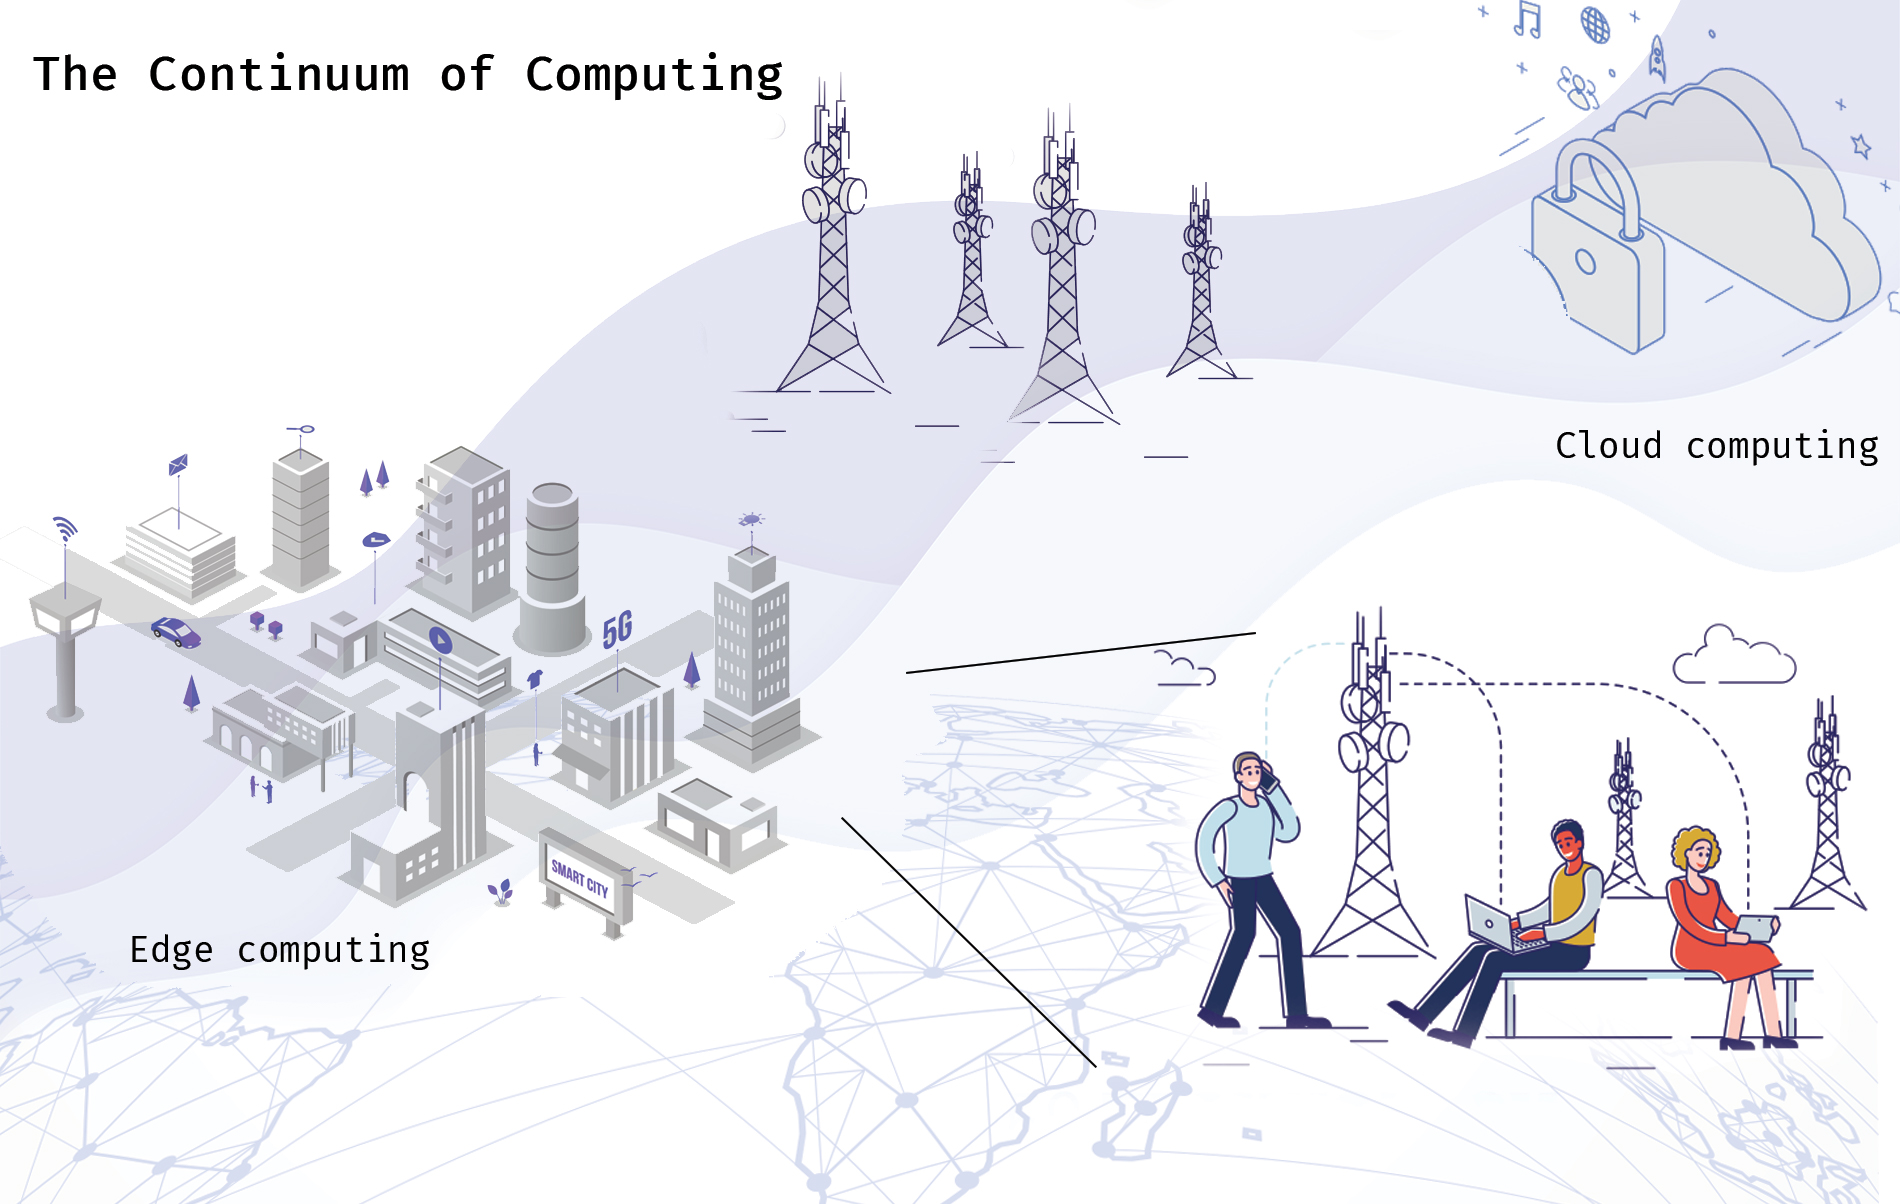
\includegraphics[width=0.7\textwidth]{figures/continuum}
\caption{Pictorial view of the Continuum of Computing.}
\label{fig:continuum}
\end{figure}
Enacting this vision requires that sufficient compute capabilities be deployed at the edge of the network, where physical reality begins and connected edge devices operate as the bridge between the physical and the digital worlds.

The Continuum of Computing as we understand it in this paper aggregates distributed services and deploys them from across the Edge, close to data sources, through to the center of the Cloud, along the path that best serves the user need for location, response latency, and resources.
Depending on the use case and service level requirements, user applications may require processing and storage at the Edge, in the Cloud, or somewhere in between. %\textcolor{red}{Fog computing \cite{fog-computing} is the term coined by the research community to identify computational resources situated at a few, usually one, hop away from end users. Figure~\ref{fig:continuum} depicts Fog nodes as base stations, which users connect to in everyday activities.}
%This paper puts forward a vision that follows naturally from the previous premises - the \textbf{Continuum of Computing} - a ubiquitous platform where distributed on-demand resources and services on the whole computing continuum are dynamically provisioned to support different ranging services and released with minimal management effort.

The foundation of the Continuum is made up of pervasive service platforms located anywhere the user is and a multitude of services, with different granularity, available over the Internet and composed opportunistically according to user needs.
%The service providers offer services, and consumers use them to accomplish any high-level application-specific goal. Services should be composed of other existing services, leveraging the principle of reuse. These services' granularity can be very different, ranging from high-level business to low-level sensing provided by the Internet of Things.
%\textcolor{red}{In essence, the Continuum is constituted by software and hardware resources provided as-a-service, which can be delivered anywhere the user is, independent of their respective location. }
The Continuum must facilitate the elastic provisioning of the end-to-end service delivery infrastructures virtualised to allow scaling as a function of user demand and service requirements. 

With \cite{latre2014fluid}, \cite{abdelbaky2017computing}, and \cite{beckman2020harnessing}, we envision the Continuum to behave as a fluid, which continuously adapts its shapes to fit the environment where computation may freely flow \textit{beyond} merely connecting network nodes to allow computation to happen at predetermined locations in the computing space.
%The notion of Continuum of Computing is not entirely novel: the authors of \cite{latre2014fluid} did envision a Fluid Internet, which "seamlessly provisions virtualised infrastructure capabilities, adapting the delivery substrate to the dynamic requirements of services and users, much like a fluid adapting to fit its surroundings". 
%This vision In a similar vein, the authors of \cite{abdelbaky2017computing} present the notion of computing in the continuum as "a fluid ecosystem where distributed resources and services are programmatically aggregated on-demand to support emerging data-driven application workflows". 
%Likewise, the authors of \cite{beckman2020harnessing} define the Continuum of Computing and seek to develop approaches that include it into a collective whole.

%\textcolor{red}{The vision of Continuum would not be feasible without the groundwork previously done in the thriving research areas of Cloud Computing and IoT. Recent works such as \cite{botta2016integration} focus on integrating the Cloud and IoT while keeping them as distinct spaces where the latter sends data and offloads computation to the former.}
%The few publications mentioned in the previous paragraph are the only ones that envision a Continuum of Computing which encompasses the whole Internet as a substrate for ubiquitous service delivery. 

Highly distributed networks are the most effective architecture for the Continuum, particularly as services become more complex and more bandwidth-hungry. Although often perceived as a single entity, the Internet is actually composed of a variety of different networks. 
The net result of such articulation is that content generated at the Edge may have to traverse multiple networks, crossing peering points before reaching its destination data center, at the center of the Cloud.
%\textcolor{red}{Unfortunately, inter-network data communication is neither an efficient nor reliable operation and can be adversely affected by a number of factors.}

\begin{figure}[ht]
\centering
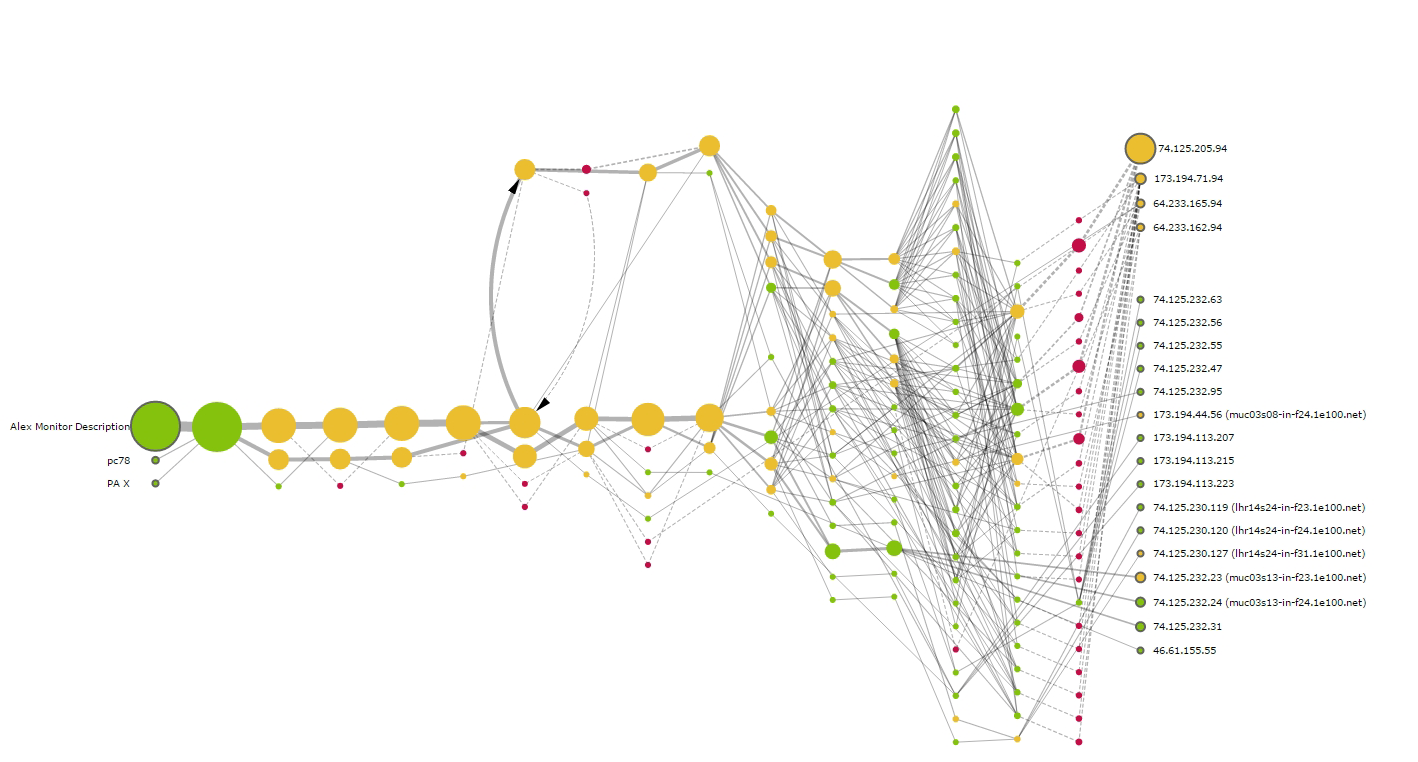
\includegraphics[width=\columnwidth]{figures/traceroute}
\caption{Traceroute virtualisation of an IP packet reaching google.com. The left green nodes are the source nodes, while packets travel across to the extreme right to servers located in data centers. Source: \cite{traceroute-google}.}
\label{fig:traceroute}
\end{figure}

The peering points, depicted as nodes in Figure~\ref{fig:traceroute}, where networks exchange traffic, are the common bottleneck of the Internet. Capacity at these points typically lags behind the reliability demand mainly due to the economic structure of the Internet \cite{nygren2010akamai}. The economic incentive ramps at the first (cloud data centres) and the last mile (IoT) of the path, with very little interest to invest in peering points, which become the cause for packet loss and increased latency.

%\textcolor{red}{Across the Internet, outages happen all the time, caused by a variety of reasons such as cable cuts, misconfigured routers, DDoS attacks, power outages, or natural disasters. While failures vary in scope, large-scale occurrences are not uncommon \cite{aws-outage}.}

For the Continuum, the throughput of the entire communication path, from IoT devices to data centres back to end users, is a paramount concern, which suggests preferring processing at the Edge to causing network pressure. 
%The bottleneck is not likely to be at just the extreme ends of the path. It could be at a peering point, as mentioned, or due to the network latency between server and device. 
%\textcolor{red}{Autonomous vehicles are an evident example of these issues. One Gigabyte of data will be generated by autonomous cars every second, which requires real-time processing for the vehicle to make correct decisions~\cite{shi2016edge}. 
%When many vehicles are to be in one confined area, such an arrangement challenges the network bandwidth and threatens reliability. 
%Moreover, if all the data were sent to the Cloud for processing, the response time would be much too long. 
%In such cases, to decrease service latency and network pressure, the data needs to be processed at the Edge.}
Offloading some compute tasks from IoT sensor or actuator nodes to the Edge is likely to be more energy efficient. 
%\textcolor{red}{Even mobile phones would enjoy significantly reduced energy consumption in that manner, especially for tasks like Mobile Augmented Reality~\cite{baresi2017empowering}.}
%\textcolor{red}{Alternate models such as Fog and Edge computing \cite{fog-computing,shi2016edge} have emerged in recent years to respond to the idea of processing the information at the nearest place. 
%A Fog and Edge-based platform, with servers anywhere the end device, can achieve the scale needed as well. 
%Each location supports higher orders of throughput, low response times, and higher energy efficiency.}
This strategy may not always be as convenient, though. Long computations, as in big-data analysis for instance, in fact, are best offloaded to a more capable but distant node, possibly up to the center of the Cloud. 
Response time is the sum of two components: the compute latency and the transmission latency. High compute latency can outweigh transmission efficiency. 
Hence, Edge computing has the responsibility to determine the preferable trade-off between the two, leveraging resources across the whole Continuum to achieve the best optimisation on a case-by-case basis.

%\textcolor{red}{Similar attention must be paid to the energy issue. 
%The battery is the most precious resource for things at the edge of the network, but wireless communication module is usually very energy-hungry \cite{shi2016edge}. For a given workload, it is not always the case that the most energy-efficient solution is to offload the whole workload to the Cloud rather than compute it locally. 
%Once again, the key is the trade-off between compute energy and transmission energy. Offloading to another node is preferable only if the latter overhead is less than that of computing locally.}

Determining the best location for the computation to happen dynamically, requires seamless movement of data and computation. Such Continuum is not one form of computing (e.g. edge computing) supplanting another (e.g. cloud computing), but an evolution that harnesses the entire computing space as a whole.

\paragraph{Contribution}
No matter how attractive this vision may be, however, very little efforts have been carried out to date, to the best of the authors' knowledge, to explore the development of suitable enabling platforms. The work discussed in this paper aims to fill this gap. 

\textcolor{orange}{Inserire qua anticipazione delle conclusioni dove diciamo che questo lavoro esplora la fattibilità pratica del Continuum allo stato dell'arte di alcune pertinenti tecnologie.
Dobbiamo anche dire dove discutiamo lo stato dell'arte intorno agli argomenti che trattiamo.}

The remainder of this paper is organised as follows. Section \ref{sec:challenges} presents the challenges resulting from realizing the envisioned Continuum of Computing. 
Section \ref{sec:technicals} shows the problem space addressed by this paper and the technology baseline. 
Section \ref{sec:evaluation} contains an evaluation of the architecture presented in the preceding section.
Section \ref{sec:conclusion} draws conclusions and outlines future work.

\section{The challenges ahead}
\label{sec:challenges}

We acknowledge that several challenges lay ahead in the realization of the Continuum as we have described it. 
Besides featuring extreme heterogeneity, in fact, current Edge technology most notably lacks support for service orientation, interoperability, orchestration, reliability, efficiency, availability, and security.
While not exhaustive, we deem this list of required features a decisive enabling factor.
To understand these needs and relate the experimental findings discussed in Section \ref{XXX} to them, we now briefly discuss each such requirement in isolation. 

\paragraph{Context-sensitive service orientation}
We deem service orientation the most appropriate style to organise and utilise distributed capabilities that may lie under the control of different ownership domains. 
% A Service-Oriented Architecture (SOA) provides "a uniform mean to offer, discover, interact with and use capabilities to produce desired effects consistent with measurable preconditions and expectations" \cite{mackenzie2006reference}.

A service-oriented model is centered around a service provider that publishes its service interface (i.e., how users may access the corresponding functionalities) via a service registry where consumers may locate it and use it to bind to the desired service provider \cite{haller2008internet}.

The prime virtue of such a model is the loose coupling it earns for services, which are solely responsible for the logic and information that they encapsulate, agnostic of the composition in which they can be aggregated by higher-level providers, and placed behind well-defined interfaces and service contracts with corresponding constraints and policies.
This design is in stark contrast with the dominant practice of present day, where a multitude of ad-hoc programs are developed that are confined to single places of the network, and permanently fix the behavior of the associated devices \cite{beckman2020harnessing}.

However, major limitations have to be overcome before services can be operated seamlessly and maintained agilely.  

First and foremost, the lack of vendor-neutral, trustworthy and widely accepted service intermediaries, to enable efficient retrieval of services that meet given user needs and warrant agreed levels of quality. Unfortunately, to date, interoperability is not dear to the main actors in the field \cite{grozev2014inter}.

Secondly, the lack of inter-operable support for composing higher-order services from lower-level ones. 
Individual providers adopt their own conventions for interfaces and communication protocols: for example, Google Cloud Platform services heavily use Protocol Buffers \cite{protobuf}, a Google technology for serialising structured data, in their service APIs. 
A plausible implementation of the Continuum would have to map high-level descriptions (e.g., flexible key-value stores) to vendor-specific implementations.

Moreover, whereas services on the Internet of today are mute and unresponsive, future services should be communicative and reactive to their respective environments~\cite{haller2008internet}. 
The current service interfaces in fact are ostensibly designed with human interaction in mind, thus being scarcely suited for machine-to-machine (M2M) discovery and interaction. 
%\textcolor{red}{Recent REST community efforts have begun to address this need~\cite{openapi}.}

In our vision of the Continuum, binding a consumer to a particular service interface should entail minimal direct interaction with the provider's infrastructure: the provider should have complete control of the service, relieving the customer from any associated cost of ownership.

Finally, services fit for the Continuum, hence deployable at the Edge, should be sensitive to the context of the environment in which they operate.
The context awareness we envision would help implement local control loops and trigger specific actions on local events (such as sensor readings, for instance).

\paragraph{Orchestration}
The transition to the Continuum will require coordinating and scheduling the operation of myriads of distributed service components. The complexity of that endeavor will make orchestration essential, over and above the rating it enjoys from DevOps adopters~\cite{nygren2010akamai}. 
Granted, orchestrating in the Continuum is especially challenging owing to the scale, heterogeneity and diversity of resource types, and the uncertainties of the underlying environments for resource capacity (e.g. bandwidth and memory), network failures, user access pattern (e.g., for quantity and location), and service life cycle.
Extreme heterogeneity also hinders devising sound pricing models that reflect account locations, resource types, transport volumes, and service latency.

Orchestrating services in the Continuum is a remarkable challenge, which encompasses technologies from a variety of fields, including wireless cellular networks, distributed systems, virtualization, platform management, and also requires mobility handover and service migration at local and global scales.

\paragraph{Virtualisation}
\label{sec:virtualisation}

The rapid pace of innovation in data centers and application platforms has transformed the way organizations build, deploy, and manage services.
Container-based virtualization, owing to its natural versatility and light unitary weight, has become the dominant solution for all seekers of elastic scalability.
%\textcolor{red}{Born off Linux Containers (LXC)~\cite{bernstein2014containers}, modern containers are an OS-level virtualisation solution for running multiple isolated applications that all share a common underlying Linux kernel. 
%A container consists of one or more processes with reduced privileges and restricted visibility into kernel objects and host resources.}
Thousands of containers can be stored on a physical cloud host in contrast with just very few traditional heavy-weight Virtual Machines. 
A near-future can be hypothesized where Edge-friendly containerization will allow users to deploy services and applications on heterogeneous Edge nodes with minimal effort. 
Several works (e.g. \cite{pahl2016container} and \cite{bellavista2017feasibility}) argue the feasibility of container virtualisation applied to cheap low-powered devices, such as the Raspberry Pi~\cite{raspberry}.
Thanks to the underlying Docker image technology \cite{docker-image}, containers provide resource isolation, self-contained packaging, anywhere-deployment, and ease of orchestration, very fitting features for the Continuum.
Several Cloud providers use this technology for their Platform-as-a-Service and Function-as-a-Service solutions.

Modern serverless~\cite{jonas2019cloud} platforms (e.g., Google Cloud Functions~\cite{gcloud-functions}, Azure Functions~\cite{azure-functions}, AWS Lambda~\cite{aws-lambda}) isolate functional units in ephemeral, stateless containers. 
Using containers, however, incurs latency between hundreds of milliseconds and seconds~\cite{mohanty2018evaluation}, wholly unaffordable for latency-sensitive services that operate at the Edge. 
To achieve better efficiency, some platforms cache and reuse containers across multiple function calls within given time windows, typically 5~minutes. 
In the Edge, however, long-lived and over-provisioned containers can quickly exhaust local resource capacity, and become impractical for serving multiple IoT devices. 
Supporting a large number of serverless functions while warranting low response time, within tens of milliseconds~\cite{elbamby2019wireless}, thus is one of the main performance challenges for resource-constrained Edge nodes.

In the way of hard security, containers offer weak isolation. To achieve stronger guarantees, they are often run in per-tenant virtual machines, too heavy for Edge or Fog nodes. 
A light\-weight yet robust isolation solution thus is a hot research question in the quest for the Continuum.
%\textcolor{red}{Interesting lightweight isolation platforms such as Firecracker and gVisor~\cite{caraza2020blending}, have come to light recently, as a bridge between containers and full system virtualization. 
%Firecracker provides a narrower interface to the host kernel by starting minimal guest VMs and providing full virtualization. gVisor has a wider interface, instead. 
%Both have low memory overhead and decent start-up latency.}

%\textcolor{red}{Unikernels~\cite{madhavapeddy2013unikernels}, which combine a minimal OS and a single application, are another novel virtualization technique of potential interest to the Continuum. Experiments with Unikernel-based serverless functions show 6x better latency and throughput than for mainstream solutions~\cite{koller2017will}. 
%Unfortunately, Unikernel implementations currently lack the maturity needed for production (e.g., assist tooling, decent ecosystem, and aids for non-expert users). This disadvantage makes porting containerized applications very challenging. }

Interestingly, the basic units of execution in the as-a-service world have continuously shrunk in size and codebase over the last few years: from VMs to containers and serverless functions (which are currently built into vendor-specific container images behind the scenes).
A direct consequence of that, modern applications are already comprised of an increasingly large number of small distributed components.

\paragraph{Dynamic configuration}

Edge and IoT nodes must be capable of prompt reaction to context changes in the environment where they operate. 
Such reactions are critical to applications like video analysis~\cite{jang2018application} that are natural candidates for deployment at the Edge. 
The risk scenario to be avoided is that IoT devices continue to operate needlessly or erroneously because their controllers running on nearby Edge nodes are late in making opportune adjustments.

Enabling dynamic configuration on constrained devices would allow swift adaptation to environmental events in accord with application requirements. 
This goal can be achieved by running an application-specific computation on the node itself, earning a considerable improvement in task accuracy (owing to physical vicinity), network bandwidth, and response time.

Opening Edge devices to arbitrary code execution, though, exposes the system to malicious acts, with compromising breaches that can exploit the slightest code weakness.
Current software isolation stacks can hardly be used in trustworthy embedded systems as they may lack dual-mode protection hardware, storage capacity, or OS components~\cite{peach2020ewasm}. 

A further challenge of dynamic configuration is to strike an acceptable compromise between warranting isolated execution and containing the corresponding loss of efficiency and increase in energy consumption. 
A common memory-safe execution technique is to adopt interpreted languages that provide type and memory safety. 
For instance, the authors of \cite{brzoza2016embedded} have ported interpreters of high-level languages (Lua and Python) to C to support dynamic reconfiguration of the internal logic in telemetry sensors.

\paragraph{Interoperability}
\label{sec:interoperability}

Many technologies are available for connecting and integrating all kinds of "things" into the Continuum. 
ZigBee, IPv6 over Low-Power Wireless Area Networks (6LoWPAN), MQTT, and CoAP~\cite{naik2017choice}. are popular in the wireless sensor networking area, while OPC \cite{gruner2016restful} has a good take-up in factory automation. 
The fact is, though, that such technologies are too numerous and varied for any single standard to be able to accommodate all of them.

For this reason, building the Edge infrastructure of the Continuum requires coping with extreme heterogeneity, which standards will hardly be able to tame.
Best is to separate functionality from implementation, thus seeking interoperability in lieu of standardization. Service-oriented architectures are ideal in this regard as they encapsulate functionality in services that can expose a common interface, abstracting away inner idiosyncrasies.

Having an infrastructure that allows connecting and integrating a diverse set of technologies is not just a "necessary evil" but rather a strength that earns two key benefits. Firstly, it allows applying different solutions to different applications, in a best-fit logic. 
%Depending on the application requirements, the best-fitting technology can be used.
Secondly, an infrastructure where diverse technologies can easily be integrated into will be more future-resistant. 
This is particularly important for the Edge and IoT, which are still in their infancy, and will certainly see new developments for technologies and protocols. An infrastructure built with technology diversity in mind will allow interoperability with existing and already deployed devices and networks.
%\textcolor{red}{A similar level of heterogeneity occurs for Cloud platforms, which typically expose proprietary interfaces in isolated vertical solutions, which very much hamper cross-platform resource integration~\cite{grozev2014inter}. }

\paragraph{Portability and Programmability}
In Cloud-native models of computing, users of containerization are free to elect the programming language of choice, with the sole concern to ensure that the corresponding executable image, which embeds all the necessary package libraries and configurations, can be deployed on the target platform. 
Such images can be constructed from minimal file system layers, sharing read-only parts of them, notably the base OS, with other containers, thus shedding considerable footprint. 

Conversely, in the Edge and, by extension, in the Continuum, the compute nodes are vastly diverse for CPU (e.g., x86\_64, ARM32, ARM64, and RISC-V) and runtime, which makes it much harder for programmers to make application development and deployment decently portable. 

Docker images attempt to overcome this challenge by defining multiple variants (usually referred to as tags) of the same image, to target multiple architectures, for processor or OS. 
This nice feature, however, does not alleviate the pain of configuring and building each application image for each target platform. Moreover, the lack of general-purpose OSs embeddable on Edge devices or their limitation in resource capacity prevent from using conventional containers on them, further impairing portability across the Continuum.

Portability also relates to programmability, in that the choice of programming language may favor or hinder portability. 
%  \textcolor{red}{To facilitate data processing at the edge of the network, the authors of~\cite{shi2016edge} propose computing stream defined as a serialization of functions applied along the data propagation path. Likewise, the work in~\cite{beckman2020harnessing} proposes a simple Function-as-a-Service abstraction that allows pushing new algorithms and Deep Learning models to the desired network location, that is, Edge, Fog, Cloud, HPC farm.}

The Serverless paradigm fits this bill well on two grounds~\cite{yi2017lavea}. First, the serverless programming model makes  developing, deploying, and managing applications dramatically less burdensome than in conventional styles.
Second, individual functions may flexibly and equally run on the Edge or the Cloud alike, thus earning much in the way of portability.

However, while well suited for event-driven and request-reply applications, the serverless computing model falls short for long-running services that must feature high availability and low latency, as needed for Edge-based user interaction or industrial control loops.
 
%\textcolor{red}{Batch jobs such as in scientific computations or MapReduce applications~\cite{condie2010mapreduce}, which are not recurrent, are often short, and are more lenient toward performance fluctuations, are more suitable to run on the Cloud. 
%However, some authors praise the benefit of running big-data analysis on the edge~\cite{he2017multitier}, notably for latency reduction.}

\paragraph{Mobility}
In the Continuum, services should be relocated following the user's movements, and so should the corresponding data and state. 
It therefore follows that all synchronization, data \& state migration, handshakes and collaboration needs have to be addressed across multiple layers of the compute and communication infrastructure.
When mobility is involved, provisioning data and services ought to be highly reactive and highly reliable, which is a challenge. 
For example, present-day vehicular networking and communication reportedly appear to be intermittent or unreliable~\cite{he2014developing}.

\paragraph{Security and Privacy}

The seamless integration of Edge, Fog, and Cloud computing is bound to raise unforeseen security issues. Previously unexplored scenarios, such as the interplay of heterogeneous Edge nodes and the migration of services across global and local scales, create the potential for original channels of malicious behaviour~\cite{yu2017survey}.

In point of principle, end-user data originated at the Edge should be stored locally, with the user able to control whether and which service providers be allowed to access them. 
As long as Edge nodes expose vulnerabilities (e.g. tampering, spoofing, falsifying), however, storing and processing privacy-sensitive data there should be regarded as far more hazardous than retreating them at the center of the Cloud.

\section{System design}
\label{sec:technicals}

After itemizing the challenges of the Continuum as a concept, we now draw a reference architecture for it as a single, unitary, and coherent software system.
Subsequently we pick a selection of specific state-of-the-art technologies that we regard as suitable candidates for its realization, and highlight the difficulties that we encountered. 

\subsection{Cluster federation}

\begin{figure}[ht]
\centering
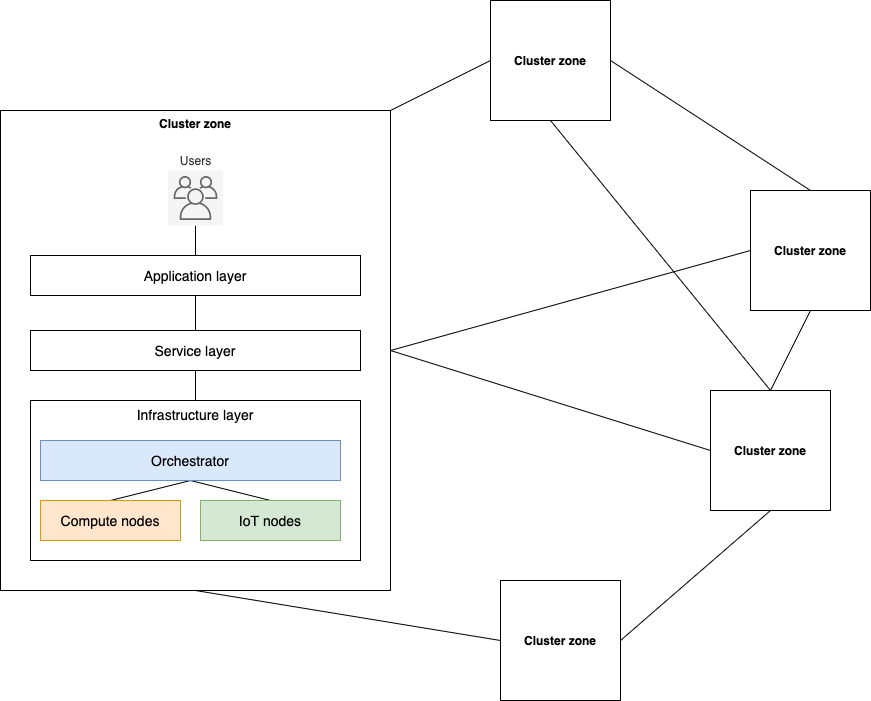
\includegraphics[width=0.75\columnwidth]{figures/architecture-federation}
\caption{A high-level view of a federated set of cluster nodes.} \label{fig:architecture-federation}
\end{figure}

As shown in Figure~\ref{fig:architecture-federation}, 
the basic building block of the system is a \textit{cluster node} amenable to a flexible, agile, and geographically bound aggregate called \textit{cluster zone}.
Each such zone federates the resources collectively available within its nodes, and orchestrates their deployment. 
%The rationale for a federation layer is two-fold.

The federation is achieved via a dedicated \textit{infrastructure layer}, which discovers and aggregates services, data and compute resources transparently across cluster nodes in a manner that meets end-to-end QoS requirements.

The system as we envisage it, dynamically instantiates and schedules services along the path from source to destination, based on application-specific requirements and constraints. 
In the event that a single cluster zone lacks hardware, software or data resources to meet the user needs, it would propagate the corresponding requests outside of its federation to cluster zones within an acceptable geographical distance that have the required capabilities.

Collaboration among cluster zones is essential to support user mobility across neighboring regions. 
In the Continuum, services should follow the user movements without significant outage or perturbation.

User applications running on a single cluster node access resources thanks to the intermediation of the \textit{service layer}. Applications intending to run on a cluster zone specify their service requirements and constraints, namely the type of resource (e.g., expected performance, pricing), without detailed knowledge of the underlying infrastructure. 
The \textit{orchestrator} receives the requirements from the \textit{service layer} intermediary, and provisions resources and services as required, assigning them to \textit{compute nodes} in the target cluster zone.
While geographically distant, such nodes form an interconnected cluster that logically aggregates the available resources.

% \textcolor{red}{Applications are described as manifests, which itemize the relevant resources and service requirements.
% Resources concern for example the amount of CPU and memory.}
Services capture common dependencies like a database and persistent storage for data sources, along with pertinent constraints on them, such as latency limits and subscription plans.

At this early stage and due to the broad scope of the topic, we leave the federation architecture as an open research question for the future of the Continuum. 

\subsection{Infrastructure architecture}

The infrastructure layer is composed of a set of service providers that offer data and computational resources. The data can be generated by streaming IoT devices (e.g. cameras, smartwatches, and smart infrastructure). 
The computational resources can be heterogeneous and distributed through the infrastructure, from the Cloud to the Edge.

\begin{figure}[ht]
\centering
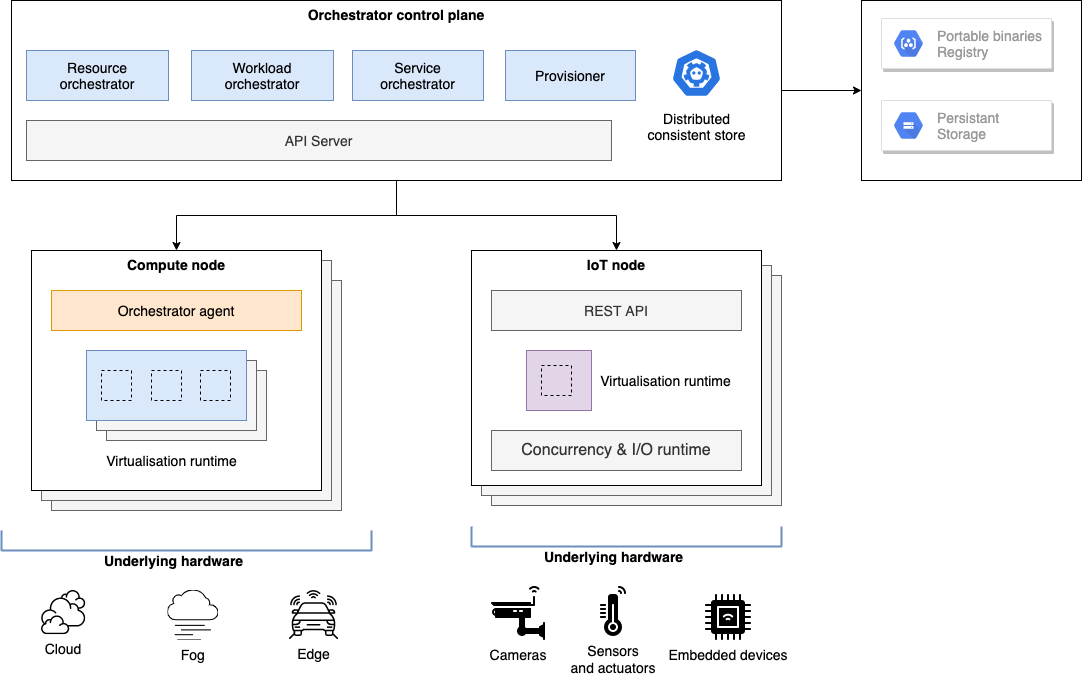
\includegraphics[width=\columnwidth]{figures/architecture-broad}
\caption{Reference architecture for the infrastructure.}
\label{fig:architecture-broad}
\end{figure}

A reference architecture of the infrastructure is shown in Figure~\ref{fig:architecture-broad}.

\subsubsection{Orchestrator control plane}

The orchestrator control plane is the core of the orchestration system. It has a resource monitor module responsible for keeping track of real-time resource consumption metrics for each node in the compute cluster. The scheduler usually accesses this information to make better optimisation decisions. The scheduler is responsible for determining whether there are enough resources and services available in the Continuum to execute the submitted application. If resources are insufficient, applications can be rejected or put on wait until the resources are freed. Another possible solution would be to increase the number of cluster nodes to place the incoming application. Such nodes may be provisioned from local machines or anywhere in the network, typically close to the cluster. After determining if requirements can be satisfied, the scheduler maps application components onto the cluster resources. This deployment is done by considering several factors, e.g. the availabilities, the utilization of the nodes, priorities, or constraints.

In cases where the addition of new cluster nodes is possible, an automatic process is necessary. The provisioner is responsible for dynamically adding nodes (physical or virtual) to the cluster when the existing resources are insufficient to meet the applications' demands. It will also decide when nodes are no longer required in the cluster and shut the nodes down to prevent additional costs.

\subsubsection{Compute nodes}

Each machine in the cluster that is available for services and applications is a compute node. Each of these nodes has an implementation of the orchestrator agent runtime with various responsibilities. First, it collects local information such as resource consumption metrics that can be periodically reported to the control plane. Second, it starts and stops service instances and manages local resources via a virtualisation runtime. Finally, it monitors the instances deployed on the node, sending periodic status to the control plane.

\subsubsection{IoT nodes}

IoT nodes are embedded devices that act as sensors and actuators, provided as services to the cluster. The IoT nodes are heterogeneous in runtime implementation and communication protocols. Therefore applications in the cluster interface with them via brokers provisioned by the cluster, as explained in Section §\ref{sec:akri}. Besides, the embedded devices support dynamic configuration by running arbitrary virtualisation modules in a lightweight runtime, assuming the module size and the hardware requirements can be satisfied by the limited device.

\subsubsection{Underlying infrastructure}

One of the main benefits of containers is their flexibility in being deployed on a multitude of platforms. Because of these, the cluster machines can be either VMs on public or private cloud infrastructures, physical machines on a cluster, or even mobile or edge devices, among others.

\section{Addressed challenges}

In this work, we propose and have implemented a Proof-of-Concept (POC) concrete technology baseline for the cluster nodes of the Continuum. Notably, the POC's goal is to prove that the technologies can be integrated to support the realisation of the Continuum's infrastructure layer and evaluate their maturity for such a goal.

The authors of \cite{balouek2019towards} do describe a similar framework to combine heterogeneous resources from the edge to the cloud. However, the cited concept is focused on stream-oriented workflows and real-time distributed data processing. A novel point of this work is the focus on a general-purpose solution capable of supporting a wide range of services. 

We proceed to provide some groundwork on how to address the following challenges within the list discussed in Section §\ref{sec:challenges}. For each of the following points, the paper presents a candidate technology that is intended to show an evaluation of its fitness in the overall system:

\begin{enumerate}
    \item \emph{Service orientation}: the web architecture is proposed as the substrate for the pervasive communication between services in the Continuum, and the Representational State Transfer (REST) (§\ref{sec:web}) is the natural architectural style to follow so that services can communicate uniformly. Furthermore, we present the Open Service Broker (§\ref{sec:osb}) platform to allow independent vendors and developers to provide services running on popular service orchestrators;
    \item \emph{Orchestration}: Kubernetes (§\ref{sec:kubernetes}) is proposed as an orchestrator for resource orchestration, workload orchestration and service orchestration of the Continuum. On this matter, Akri (§\ref{sec:akri}) extends Kubernetes to support the orchestration of IoT devices with an attempt to overcome the heterogeneity and unreliability of the underlying environment;
    \item \emph{Virtualisation}: WebAssembly (§\ref{sec:webassembly}) is used as platform-agnostic virtualisation technology to provide lightweight sandboxing capabilities on every node of the Continuum. WebAssembly is a portable bytecode that is a compilation target of potentially any programming language;
    \item \emph{Dynamic configuration}: the combination of a small WebAssembly interpreter and the low-overhead binary format of the bytecode result in intriguing opportunities for dynamic configuration of IoT devices;
    \item \emph{Interoperability}: REST is a natural choice to support high-level interoperability between services as well. The CoAP (§\ref{sec:coap}) protocol exposes constrained devices' capabilities as REST resources. Such resources are then made available within the Kubernetes cluster, easily accessible as RESTful services. Akri's broker-based architecture offers a compelling solution to the heterogeneity of the Internet of Things. Similarly, the Open Service Broker allows a similar opportunity to work around the interoperability issue between cloud providers via a broker-based architecture;
    \item \emph{Portability and Programmability}: we propose using the latest standard for Docker images to support the distribution of arbitrary binary files, notably WebAssembly applications instead of container filesystems. This solution significantly improves the integration with existing development tools and lowers the entry barrier for developing applications in the Continuum. Lastly, we mention the notable role of the Rust (§\ref{sec:rust}) programming language and its value for for both service providers and application developers because of its modern language features, the security guarantees and its tight integration to the WebAssembly technology;
\end{enumerate}

% \textcolor{red}{Due to the ample problem space, mobility, security and privacy are not addressed in this paper and are left as open research questions. Besides, by any means, it is also not in the intentions of this paper to be assertive in the technical solutions proposed here. This work intends to present a snapshot of today's technology to evaluate the distance between state of the art and the continuum vision.}

Figure~\ref{fig:architecture-technologies} presents the key technologies mentioned above within the reference architecture of the infrastructure.

\begin{figure}[ht]
\centering
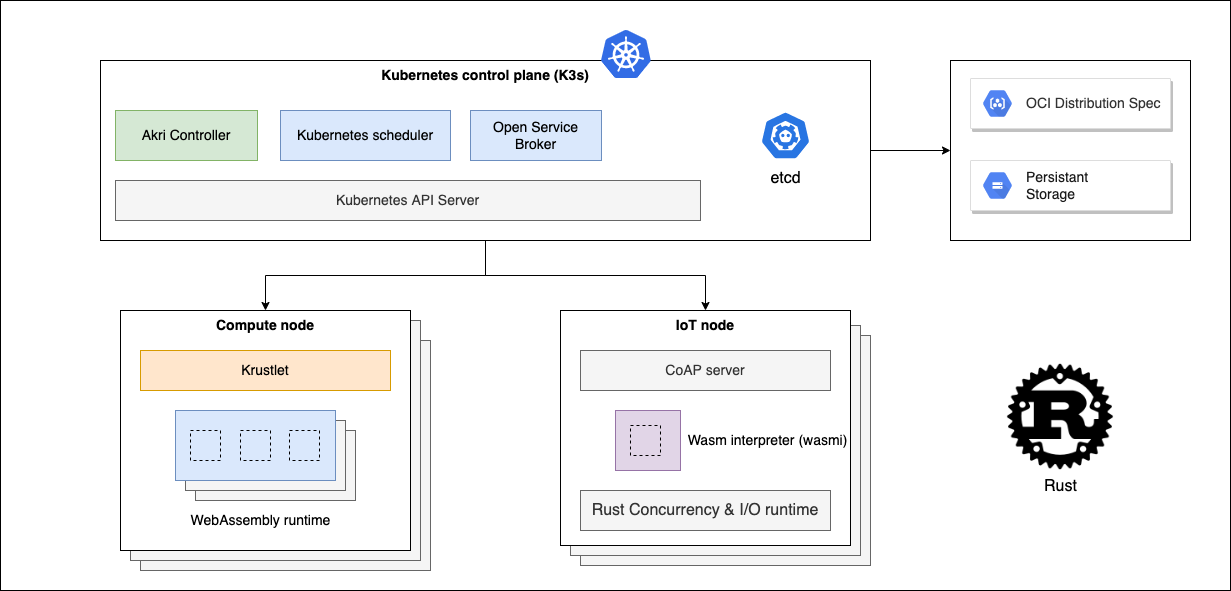
\includegraphics[width=\columnwidth]{figures/architecture-technologies}
\caption{Technology baseline for the reference infrastructure architecture. \textcolor{orange}{Togliere RTIC dall'immagine.}} \label{fig:architecture-technologies}
\end{figure}

\subsection{Web services}
\label{sec:web}

%  \textcolor{red}{Tim Berners-Lee's original vision for the web focused on documents and their inter-relationships, but it has become more and more a web of applications in the last decade. Nowadays, } 

the web has become the world's most successful vendor-independent application platform.

The web is a loosely coupled architecture and applications today depend on the web architecture, using HTTP to access information and perform updates. The most dominant architectural style is Representational State Transfer (REST) \cite{rest} that makes information available as resources identified by URIs. Applications communicate by exchanging representations of these resources using a transfer protocol, HTTP, precisely. HTTP is the most popular application protocol on the Internet and the pillar of web architecture. However, new communication protocols (e.g. CoAP in Section \ref{sec:coap}) are emerging to extend the web to the Internet of Things and HTTP itself is undergoing revisions (e.g. HTTP/3 or QUIC \cite{langley2017quic}).

The prime traits of REST that make it an enabler for the Continuum are as follows:

\begin{itemize}
    \item Resource orientation: resources are an information abstraction that allows servers to make any information or service available, identified via Uniform Resource Identifiers (URIs). The REST architecture allows the server to own the original state of a resource, and the client negotiates and accesses a representation of it. The representation negotiation is suitable for interoperability, caching, proxying, and redirecting requests and responses. Such features enable seamless inter-operation of services in the Continuum through proxies, scalable architectures and better availability. Besides, under the REST architecture, web resources often advertise links to other resources creating a distributed web and resulting in an even more scalable and flexible architecture;
    \item Uniform interface: clients access these server-controlled resources in a request-response fashion using a small uniform set of methods with different semantics (GET, PUT, POST, and DELETE). The requests are directed to resources using a generic interface with standard semantics that intermediaries can interpret. The result is an application that allows for layers of transformation and indirection independent of the information origin;
    \item High-level interoperability: besides the representation negotiation, the REST architectural style enables further interoperability between RESTful protocols through proxies or, more generally, intermediaries that behave like a server to a client and play a client with respect to another server. REST intermediaries play well with the assumption that not every device must offer RESTful interfaces directly. In several cases, notably in the Internet of Things, it may not be possible to change the underlying communication protocol. However, intermediaries allow exposing the resources through a RESTful API nevertheless. The interactions behind that RESTful interface are invisible and may include highly specialized protocols for the specific implementation scenario (e.g. OPC UA or MQTT) \cite{guinard2010resource};
    \item Communication protocol independence: Public APIs benefit from the adoption of HTTP because it leads to an API accessible from all programming languages and environments without additional technology. On the other hand, HTTP is relatively expensive for both binary overhead and network resource usage. Fortunately, the REST architectural style is not strictly tied to HTTP, and new communication protocols like CoAP (§\ref{sec:coap}) can offer a very similar interface while guaranteeing more lightweight implementation, less demand for network bandwidth, lower latency and more energy efficiency among many features;
    \item Machine-to-Machine communication (M2M): communication protocols must be specifically designed for efficient M2M communications without introducing overhead in network load, delay, and data processing. In the M2M environments typical of IoT applications (and of the Continuum, by extension), devices must discover each other and their resources. New approaches from the IETF include the well-known resource path \emph{/.well-known/scheme} (RFC 5785) and the HTTP link header (RFC 5988);
    % \item \textcolor{red}{Stateless: REST requires requests from clients to be self-contained, in the sense that all information to serve the request must be part of the request. Statelessness helps applications to scale, as persisting state in a highly distributed system brings challenges like consistency and hinders support for user mobility in the Continuum space.}
\end{itemize}

% \textcolor{red}{From the previous points, it is clear that the design goals of RESTful web systems and the benefits for a decentralized and massive-scale service system align well with the field of pervasive computing. For these reasons, REST an ideal candidate to build a universal API for services and devices in the Continuum, letting developers reuse their existing skills and tools. }

\subsection{Open Service Broker}
\label{sec:osb}

\begin{figure}[ht]
\centering
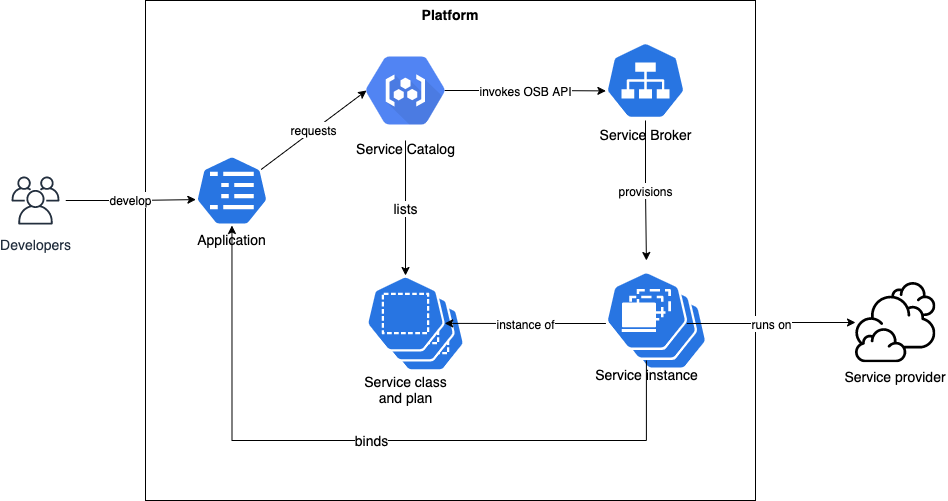
\includegraphics[width=\columnwidth]{figures/osb}
\caption{The Open Service Broker architecture.} \label{fig:osb}
\end{figure}

Managed services, whose infrastructure is handled by a vendor for the whole service lifecycle, enable developers to concentrate on their application code rather than operating these services. On this matter, on-demand marketplace services can increase developer velocity and minimise time to deliver value to the market. This idea is not novel, and the most notable example is Cloud Foundry's Marketplace \cite{cloud-foundry-marketplace}, now dismissed, unfortunately. In the Continuum's marketplace, providers control the access to the services and payment plans but allow developers to bring their own services to the catalogue. Over the years, a rich ecosystem of services will be developed and accessible via simple well-documented APIs (namely RESTful interfaces).

Contrary to this vision, cloud standards have failed to gain traction. Therefore, the need to find mechanisms for bridging the heterogeneity gap between platforms and enabling data integration is more relevant than ever. Most orchestration technologies working across administrative domains use a broker to orchestrate resources at different levels within a provider (e.g. the cloud and the edge network) and across providers \cite{grozev2014inter}. As the number of cloud vendors is limited, building adapter and brokering layers that align access to different clouds is possible. 

On this matter, several stakeholders (namely the Kubernetes community, OpenShift, IBM and Google) have shown interest and contributed to working on a standard Open Service Broker (OSB) API \cite{osb}. Components that implement the OSB REST endpoints are referred to as service brokers and can be hosted anywhere the application platform can reach them. Service brokers offer a catalogue of services, payment plans and user-facing metadata. The main components of the OSB architecture are presented in Figure~\ref{fig:osb}.

However, the actual value of the broker API is in abstracting service-specific lifecycle operations from the platform. The service broker translates RESTful requests from the platform to service-specific operations such as creating, updating, deleting, and generating credentials to access the provisioned services from applications. Service brokers can offer as many services and plans as desired. Multiple service brokers can be registered with the marketplace so that the final catalogue of services is the aggregate of all services. The platform is thus able to provide a consistent developer experience for application developers consuming these services.

\subsection{Kubernetes}
\label{sec:kubernetes}

Kubernetes \cite{kubernetes} is an open-source framework designed to manage containerized workloads on clusters and originated from Google's experience with cloud services. Figure~\ref{fig:kubernetes} illustrates the main components of the architecture.

% The basic building block in Kubernetes is a Pod. A Pod encapsulates one or more tightly coupled containers that are colocated and share the same set of resources. Pods also encapsulate storage resources, a network IP, and a set of options that govern how the Pod's container(s) should run. A Pod is designed to run a single instance of an application enabling horizontal scaling by replicating multiple Pods across the nodes. The amount of CPU, memory, and ephemeral storage a container needs can be specified when creating a Pod. This information can then be used to make decisions on Pod placement. These compute resources can be specified as both requests and limits.

Kubernetes allows for various container runtimes from a technical perspective, with Docker natively supported by the platform. Thanks to the Container Runtime Interface (CRI) API standardisation, Kubernetes supports other container technologies such as containerd \cite{containerd}.

% Moreover, etcd \cite{etcd} is an open-source highly available distributed key-value store and a fundamental part in supporting Kubernetes in managing the cluster nodes and jobs. Specifically, etcd is used to store all of the cluster's data and acts as the single source of truth for all of the framework's components.

% \textcolor{red}{Overall, Kubernetes is a highly mature system; it stemmed from 10 years of experience at Google. It is the leading container-based cluster management system with an extensive community-driven support and development base. It provides users with a wide range of options for managing their Pods and how they are scheduled, even allowing for pluggable customised schedulers to be easily integrated into the system.}

Besides the extensible scheduler, which makes Kubernetes already an intriguing choice as a potential orchestrator for the Continuum, it also supports label-based constraints for the Pods' deployment. Developers can define their labels to specify identifying attributes of objects that are meaningful and relevant to them but that do not reflect the characteristics or semantics of the system directly. An example would allow specifying that an IoT device component must be reachable from the host. Nevertheless, more importantly, labels can be used to force the scheduler to colocate services that communicate a lot into the same availability zone, improving the latency drastically and paving the way for context-aware services. % However, to realize the heterogeneity goals, it is required to filter unqualified resources continuously. New resource affinity models should be proposed to rank the resources when provisioning for different applications.

Finally, Kubernetes is also designed with multitenancy in mind, compared to Docker Swarm \cite{docker-swarm}. Docker Swarm is another popular open-source orchestrator often cited as the main competitor for edge orchestration due to its simplicity (e.g. \cite{bellavista2017feasibility}, and \cite{ismail2015evaluation}). Support for multitenancy is a must and well-aligned with their goal of executing heterogeneous services on a set of shared resources.

\subsubsection{Akri}
\label{sec:akri}

\begin{figure}[ht]
\centering
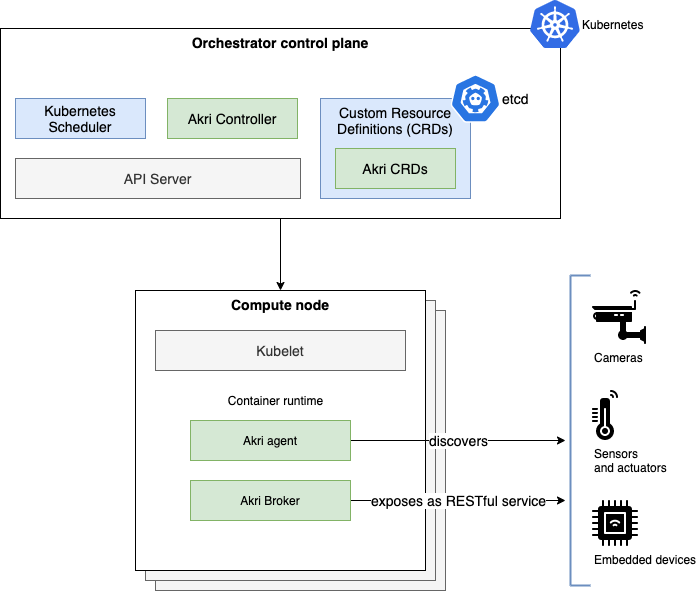
\includegraphics[width=\columnwidth]{figures/akri}
\caption{The Akri architecture.}
\label{fig:akri}
\end{figure}

Akri \cite{akri} is an open-source project which extends the Kubernetes Device Plugins API \cite{k8s-device-plugins} to allow visibility to IoT devices from applications running within the cluster. The Device Plugin API is designed initially to expose hardware resources attached to a Kubelet, such as GPUs or Solid State Drives, and it is still at the experimental stage. Akri stretched the design further so that it would be possible to implement the discovery of IoT devices, with support for the diversity of communication protocols and  ephemeral availability.

Akri's architecture, presented in Figure~\ref{fig:akri}, can be divided into four main components: the agents, the controller, the brokers and the configuration. A configuration is a Kubernetes Custom Resource Definition (CRD) to extend the Kubernetes API with new types of resources. Specifically, a configuration defines a communication protocol (e.g. OPC UA \cite{gruner2016restful}) and the related metadata, such as the protocol discovery parameters or the Docker image to use as agent.

The Akri agent is a Pod responsible for discovering devices according to a communication protocol. It can be easily developed and deployed to the cluster to support new protocols in the system. The agent will track the state of the device and keep the Akri controller updated with the status. At the time of writing, the project has built-in support for ONVIF \cite{onvif}, udev \cite{udev} and OCP UA \cite{gruner2016restful} discovery handlers, with an incoming proposal for CoAP \cite{bormann2012coap}.

Using Akri, the Kubernetes cluster can carry out dynamic discovery to use new resources as they become available and move away from decommissioned/failed resources. Discovering IoT devices is usually accomplished by scanning all connected communication interfaces and enlisting all locally available resources.

Akri is also responsible for enabling applications to communicate with the device and deploying a broker Pod as intermediary. The broker is any application instructed to communicate with the device. We devised the broker as a web server that abstracts the actual communication between devices and applications behind a RESTful API. Akri should automatically find all the devices in the environment and make them available as web resources. As an instance, the agent discovers the devices regularly by scanning for CoAP (Section §\ref{sec:coap}) resources.

Besides, the broker could offer local aggregates of device-level services. For example, it can offer a service that returns the combined temperature measurements of all the things connected to it at any given time.

A RESTful broker can also help scale with the number of concurrent HTTP requests by implementing highly performant cache mechanisms. The IoT resource periodically sends its sensor readings to the broker, where the values are cached locally. Each application request is then served directly from this cache without accessing the actual device, improving the average roundtrip time.

The broker architecture has the advantage of fully decoupling the leaf node from the cluster workload. It only needs to send an update packet with a frequency short enough to ensure data validity. On the other hand, the retrieved data's staleness will depend on the device's frequency of updates. Forwarding the HTTP request (adequately translated) has the advantage of always returning the most recent sensor reading when the request is processed. The cache mechanism cannot be applied for non-cacheable requests (e.g. HTTP POST) that must be sent to devices, such as turning on LEDs or changing the application state.

As many distributed monitoring applications are usually read-only during their operation (e.g. sensors collecting data), this architecture exhibits a greater scalability level. A potential goal is to enable new types of services where physical sensors can be shared with thousands of users with little impact on latency and data staleness.

\subsection{CoAP}
\label{sec:coap}

\begin{figure}[ht]
\centering
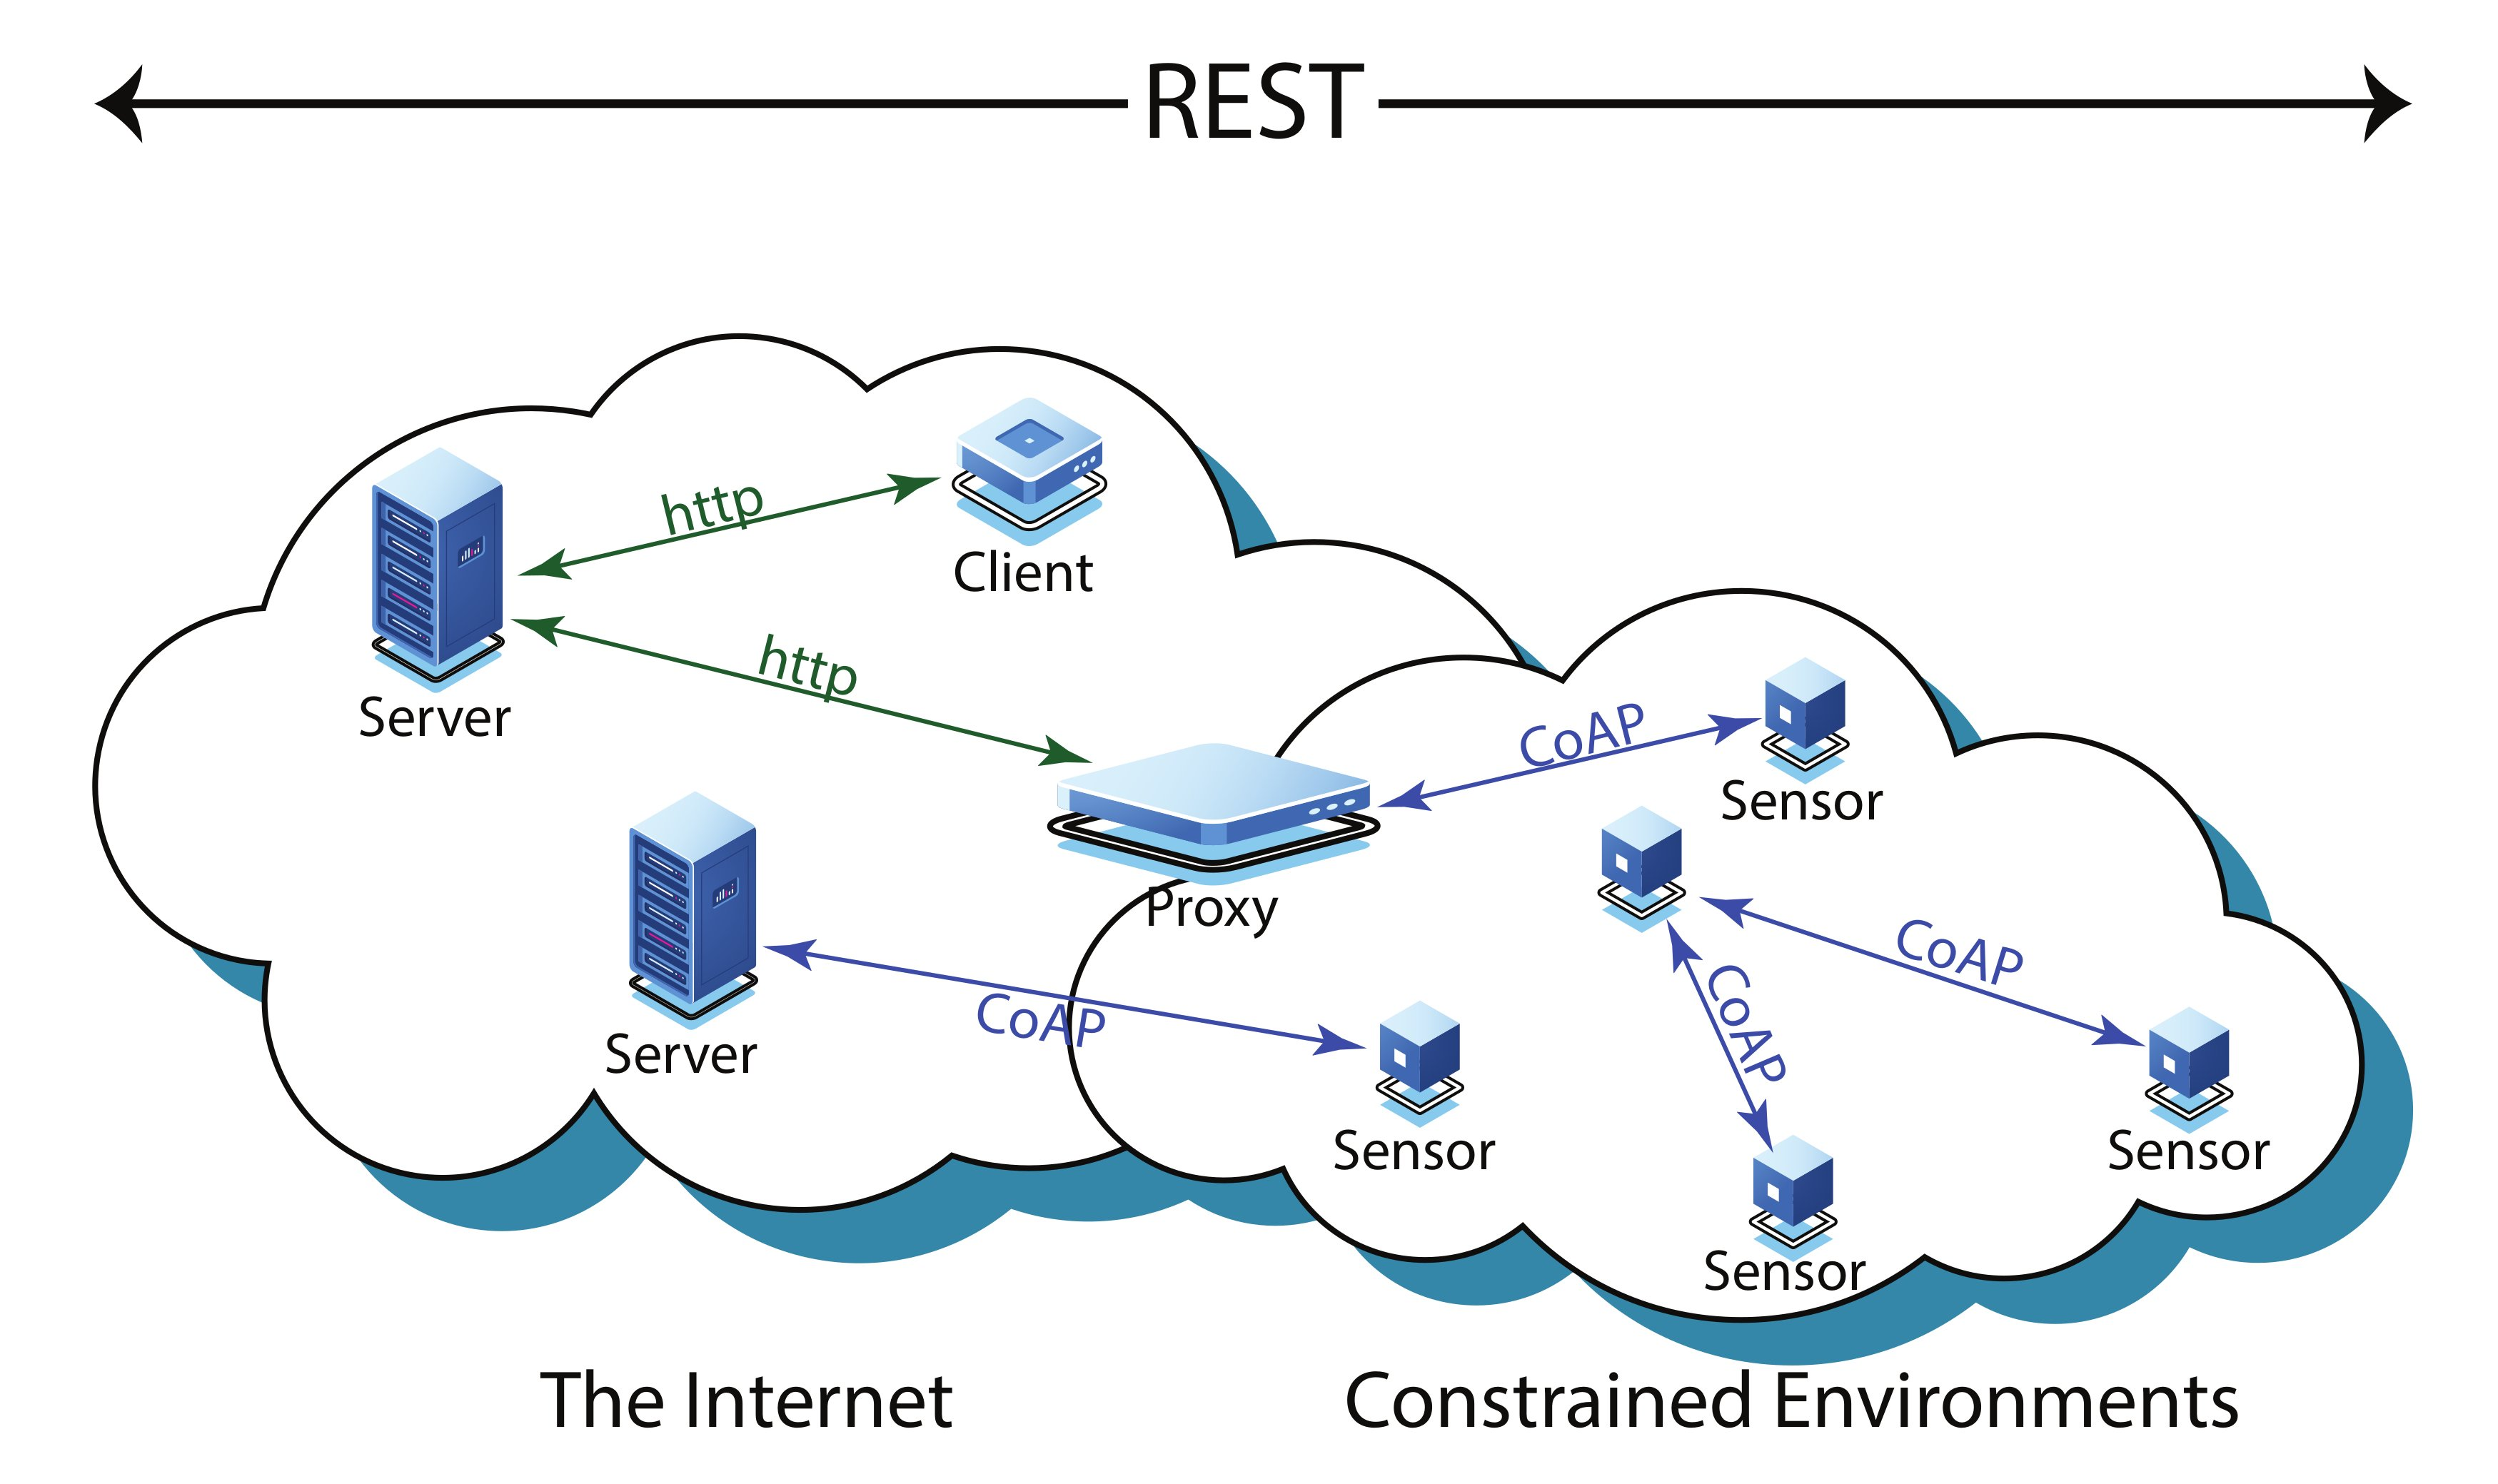
\includegraphics[width=\columnwidth]{figures/coap}
\caption{The REST architecture enhanced with CoAP. Source \cite{bormann2012coap}.}
\label{fig:coap}
\end{figure}

CoAP \cite{bormann2012coap} (RFC 7252) is a web communication protocol for use with constrained nodes and constrained (e.g. low-power, lossy) networks. The protocol is designed for M2M applications and provides a client-server architecture between IoT nodes but supports built-in discovery of resources.

A central element of CoAP's reduced complexity is that it uses the UDP transport protocol instead of TCP and defines a very simple message layer for retransmitting lost packets.
% The rationale for UDP is that TCP carries significant overhead and can have suboptimal performance for links with high packet loss, both of which are common across the Internet \cite{nygren2010akamai} and especially on remote locations where sensors might be deployed. Besides, the HTTP protocol adds further burden, as the additionally multiple round trips required for the requests can quickly add up, affecting the device performance and energy efficiency.

% CoAP uses a four-byte binary header within UDP packets, followed by a sequence of options, each up to two bytes. The protocol's specification also defines the usual four request methods: GET, PUT, POST, and DELETE. Similarly, response codes are patterned after the HTTP response codes.

The protocol is built upon key concepts of the web such as URIs and RESTful interaction \cite{pereira2013enabling}. As a result, CoAP easily interfaces with HTTP for integration with web services while meeting specialized IoT requirements such as multicast support, very low overhead and simplicity for constrained environments. 

The URI format allows exposing device data as resources and the use of standard and specialized service endpoints. For instance, CoAP servers are encouraged to provide resource descriptions via the well-known URI \emph{/.well-known/core} to achieve resource discovery. Clients then access this description with a GET request on that URI, usually via an IPv4 or IPv6 broadcast message. The description format is based on the CoRE Link Format (RFC 6690), which is simple and easy to parse. Ease of parsing allows more efficient M2M discovery and inter-communication between the nodes themselves.

% The CoAP protocol supports different resource representations, in line with the REST architecture's representation negotiation. The default format is textual for its convenience when reading and parsing. The binary format is efficient to communicate but requires external tools to make it readable by human users. XML is understandable and very well structured, but the size of its messages is significant, and it is much worse to parse than binary formats. Lastly, JSON is understandable, well structured and compact, but may still put an unnecessary parsing burden on the limited device. With all constrained devices, flash or memory consumption is one of the biggest problems, notably on devices where network connectivity already claims significant buffer memory.

Another advantage of CoAP is that human interactions follow a familiar and intuitive pattern already used by many developers by using standard web technologies. Thus, the learning curve is smoother. This feature cannot be underestimated as allowing developers to use a familiar and seamless programming experience is essential to achieve Continuum's success.

Interoperability with the rest of the Continuum can be achieved by following the REST architecture's proxy pattern, as depicted in Figure~\ref{fig:coap}. We can generally build intermediaries that speak CoAP on one side and HTTP on the other without encoding specific application knowledge. This flexibility allows deploying new applications without having to upgrade the intermediaries involved. On the other hand, an intermediary can perform the translation between CoAP and HTTP without posing further requirements either on the client or server. Because equivalent methods, response codes, and options are present in HTTP and CoAP protocols, the mapping between the two is straightforward. As a result, an intermediary (e.g. an Akri broker) can discover CoAP resources and make them available at regular HTTP URIs, enabling web services to access CoAP servers transparently.

% \textcolor{red}{However, the HTTP client-initiated interaction model may be unsuited for many event-based and streaming systems in the IoT. Data is sent asynchronously to the clients as soon as it is produced. CoAP uses the Observe approach (RFC 7641) to support pushing information from servers to clients to overcome this issue. A client can indicate its interest in further updates from a resource by specifying the "Observe" option in a GET request. If the server accepts this option, the client becomes an observer of this resource and receives an asynchronous notification message each time it changes. This kind of communication, combined with an intermediary broker, allows streaming data updates via WebSocket (RFC 6455) and overcoming the client-pull interaction model of HTTP. The broker can also help achieve more reliable communication by transparently changing the underlying sensor in case of unavailability or by avoiding closing the connection in case of temporary loss of connectivity.}

\subsection{WebAssembly}
\label{sec:webassembly}

\begin{figure}[ht]
\centering
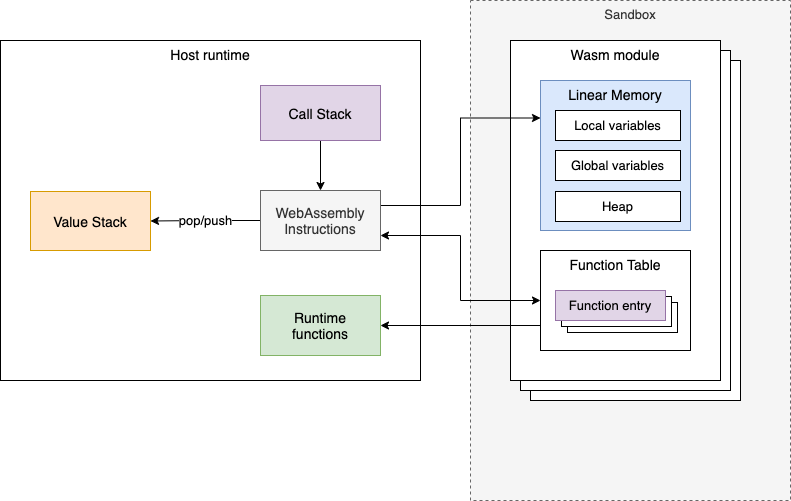
\includegraphics[width=\columnwidth]{figures/webassembly}
\caption{WebAssembly stack machine.} \label{fig:webassembly}
\end{figure}

WebAssembly (Wasm) \cite{haas2017bringing}, first announced in 2015 and released as a Minimum Viable Product in 2017, is a nascent technology that provides strong memory isolation (through sandboxing) at near-native performance with a much smaller memory footprint. WebAssembly is a language designed to address safe, fast, portable low-level code on the web. Developers who wish to leverage WebAssembly may write their code in a higher-level (compared to bytecode) language such as C++ or Rust and compile it into a portable binary that runs on a stack-based virtual machine.

% \textcolor{red}{Even though WebAssembly technically is a binary code format, it can be presented as a language with syntax and structure. This design choice was intentional since it makes it easier to explain and understand without compromising compactness or decoding ease.}

% A Wasm binary takes the form of one or more modules. It contains definitions for functions, globals, tables, and memories. 

The computation is based on a stack machine represented in Figure~\ref{fig:webassembly}: code for a function consists of instructions that manipulate values on an implicit operand stack, popping argument values and pushing result values. However, WebAssembly represents control flow differently from most stack machines. It does not offer simple jumps but instead provides Structured Control Flow (SCF) constructs more akin to a programming language. This design ensures by construction that control flow cannot contain arbitrary branches. The SCF allows WebAssembly code to be validated and compiled in a single pass as well. SCF can also be disassembled to a WebAssembly text format (.wat) that is easier to read and often overlooked but crucial human factor on the web.

A WebAssembly program's memory is a large array of bytes referred to as a linear memory or simply memory. All memory access is dynamically checked against the memory size, and out of bounds access results in a trap. Linear memory is disjoint from code space, the execution stack, and the engine's data structures. 

% \textcolor{red}{Each Wasm memory access addresses linear memory at an offset from the base, $n$, of the linear memory. Thus, some address virtualisation as an address $b$ in the sandbox is located at $b + n$ in physical memory.} The Wasm runtime is responsible for translating linear memory accesses and bounds-checking them to prevent accesses outside the sandbox.

Therefore, compiled programs cannot corrupt their execution environment, jump to arbitrary locations, or perform other undefined behaviour, especially when the original language is memory-safe (e.g. Rust §\ref{sec:rust}). At worst, a WebAssembly is subject to exploits regarding data in its memory.

This memory and state encapsulation are applied at the module level rather than at the application level, meaning that a module's memory and functions cannot leak information unless explicitly exported/returned. This granularity in sandboxing is extremely important as security incidents have increasingly exploited vulnerabilities in the dependency chain. Reuse of third-party software is pervasive in modern languages like JavaScript, Rust or Go.

The granular memory encapsulation means that even untrusted modules can be safely executed in the same address space as other code.

% \textcolor{red}{Additionally, it allows a WebAssembly engine to be embedded into any other language runtime without violating memory safety and enabling programs with many independent instances to exist in the same process.} These sandboxing features make WebAssembly a compelling technology upon which to implement a virtualisation stack for the Continuum. On the web, the substrate of the Continuum, code is fetched from untrusted sources, and it is vital that it can be safely executed on a plethora of language runtimes.

% Another critical safety feature of Wasm is the type system. Code must be validated before it can be executed safely. Validation rules for WebAssembly are defined succinctly as a type system. This type system is, by design, simple. It is designed to be efficiently checkable in a single linear pass to allow parallelisable binary decoding and compilation.
% Moreover, function pointers cannot be dereferenced directly. A call to a function pointer is translated into a function in a runtime table of valid entry points and types. The type of the function is checked dynamically against the expected type in the said entry. The dynamic signature check protects the integrity of the execution environment. In case of a type mismatch or an out of bounds table access, a trap occurs.

\textcolor{orange}{With that being said, the design goals of WebAssembly strongly advocate for its suitability for this paper}:

\begin{itemize}
    % \item \emph{Safe to execute}: \textcolor{red}{protection for arbitrary code has traditionally been achieved by providing a managed language runtime that enforces memory safety, preventing programs from compromising user data or system state. However, managed language runtimes have traditionally not offered much for portable low-level code, such as C/C++ applications, that do not need garbage collection};
    \item \emph{Fast to execute}: WebAssembly is, however, very competitive with native code, and benchmarks using Wasm runtimes on modern browsers have shown a slowdown of approximately 10\% compared to native execution and almost always within 2x \cite{haas2017bringing};
    \item \emph{Language, hardware, and platform independency}: as mentioned before, the web spans not only many device classes but different machine architectures, operating systems, and browsers. Code targeting the web must therefore be independent of any underlying hardware or platform to allow applications to run across all software and hardware types with the same behaviour;
    % \item \emph{Deterministic and easy to reason about}: WebAssembly has been designed with formal semantics from the start for both execution and validation. Besides, the Wasm binary can be compiled into a .wat file to simplify learning and debugging;
    \item \emph{Simple interoperability}: WebAssembly is similar to a virtual ISA in that it does not define how programs are loaded into the execution engine or how they perform I/O. The embedder (i.e. the host runtime) defines how modules are loaded, how imports and exports between modules are resolved, provides foreign functions to accomplish I/O, and specifies how traps are handled. It is possible, by design, to link multiple modules that different authors have created from likewise different source languages. However, as a low-level language, WebAssembly does not provide any built-in object model. It is up to developers to map their data types to numbers or memory. This design is supposed to provide maximum flexibility to developers, and unlike previous VMs like Java or .NET, it does not privilege any specific programming or object model while penalizing others. The downside of this design is that interoperability with object references is cumbersome. It involves exchanging references between the Wasm application and the host code or between modules that originated from different languages. A step in easing this issue is the recent introduction of Reference Types \cite{reference-types}. On the other hand, since WebAssembly is a virtual ISA, not over a programming language, a WebAssembly module may be compiled once and moved freely between different hardware architectures with no recompilation;
    \item \emph{Compact}: the binary code is designed to be compact. Code transmitted over the network has to be as compact as possible to reduce load times, save potentially expensive bandwidth, reduce memory usage on constrained network-attached devices and improve overall responsiveness;
    % \item \emph{Easy to validate and compile}: validation proceeds by checking on the fly while the incoming bytecodes arrive, with no intermediate representation (IR) being constructed. Benchmarks run on mainstream browsers in \cite{haas2017bringing} prove that validation can be fast enough to be performed at a full network speed of 1Gib/s;
    \item \emph{Streamable and parallelisable}: a Wasm runtime can minimise latency by starting streaming compilation as soon as function bodies arrive over the network. It can also parallelize the compilation of consecutive function bodies. For instance, each function body is preceded by its size so that a decoder can skip ahead and parallelize even its decoding. Minimising the latency is essential for increased mobility, quick release of resources, and support for low-latency use cases.
\end{itemize}

Despite the name WebAssembly, there has been a significant effort in the last years in adopting Wasm for native execution, as it is a portable target for the compilation of various high-level languages. Wasm standard does not necessarily make browser-specific assumptions, and there has been substantial work to standardize the WebAssembly System Interface (WASI) to run Wasm outside the browser. To the best of the authors' knowledge, the original design goals assumed a browser-based execution context. Nevertheless, such goals fit perfectly the Continuum's needs, where the web is the infrastructure upon which applications and services are deployed. On this matter, browsers are very much akin to an Operative System for client web applications, and WebAssembly is thus unsurprisingly being adopted on conventional OSes as well. Native execution and browser execution share many problems, like isolation, portability and interoperability, to name just a few.

At the time of writing, there are several Wasm runtimes for programs written in different languages capable of embedding Wasm applications. On the other hand, multiple compilers can compile languages to Wasm.

% \textcolor{red}{, as shown in Figure~\ref{fig:portability}. Notably, the Wasm back-end for LLVM \cite{llvm} works for C, C++, and Rust. Commercial solutions have also been slowly but steadily gaining popularity. Cloudflare's Service Workers \cite{cloudflare-workers} began to offer support for creating and hosting serverless functions in WebAssembly. In March 2019, the edge-computing platform Fastly had announced an open-sourced Lucet \cite{fastly-lucet} that provides a compiler and runtime to enable native execution of Wasm applications and can instantiate a Wasm module within $50\mu s$, with just a few kilobytes of memory overhead. Parity is also actively experimenting with writing smart contracts using Wasm \cite{parity-wasm}.}

WebAssembly is currently under experimentation as a new method for running portable applications without containers because of its design features. This method leverages its binary format as a portable vehicle to inherent memory and execution safety guarantees via its language features and a runtime with strong sandboxing capabilities. The Wasm security model enables the execution of multiple untrusted modules in the same process, thereby providing significantly more lightweight isolation compared to VMs and containers for multi-tenant serverless execution \cite{gadepalli2020sledge}.

This idea is still in its infancy, but there has been some interest in recent years, as shown by the works done in \cite{hall2019execution} and \cite{shillaker2020faasm}. All these works focus primarily on serverless computing via WebAssembly, demonstrating the popularity of such a computing model.

\subsubsection{WebAssembly for embedded microcontrollers}

An emerging use case for WebAssembly is arbitrary code execution on microcontrollers, and, as a result, interpreters are gaining popularity on resource-limited devices. wasm3 \cite{wasm3} is a popular open-source interpreter capable of running on any system with at least 64KiB of storage and 10KiB of memory. The authors of eWASM \cite{peach2020ewasm} have also explored various mechanisms for memory bounds checking and have evaluated the trade-offs between processing efficiency and memory consumption. Just-In-Time compilers for WebAssembly exist (e.g. Wasmtime \cite{wasmtime}) and receive more attention from the community, but their size and complexity make them unsuitable for microcontrollers.

Although WebAssembly interpreters can often be approximately 11x slower than native C \cite{wasm3-performance}, they help dynamically update system code and debugging but may not be applicable for code on devices susceptible to performance and energy efficiency.

In the authors' view, interpreting WebAssembly on microcontrollers remains an intriguing technology nevertheless worth the research community's attention. They offer a persuasive alternative to other language runtimes, e.g. Lua, which are commonly used on embedded devices to support dynamic configuration \cite{brzoza2016embedded}. The WebAssembly standard has many features that make it appealing for embedded devices \cite{peach2020ewasm}.

\begin{itemize}
    \item Portability: WebAssembly is a platform-independent Intermediate Representation that can be generated from different source languages and can run on many CPU architectures. Solving how to run WebAssembly on microcontrollers effectively would open the possibility to include the embedded world to the Continuum as an additional place of intelligent computing, rather than only as a mere data collector and dummy actuator;
    % \item \textcolor{red}{Broad support: there is a steadily increasingly ecosystem of vendors, tools, and languages providing WebAssembly support. With the ability to leverage WebAssembly, the embedded system community would benefit from a broader ecosystem};
    \item No mandatory garbage collection: many broadly used language runtimes such as JavaScript, Lua, or Python cannot provide predictable execution and may require excessive memory for a microcontroller;
    \item Lightweight runtime: WebAssembly mandates only a small number of runtime features around maintaining memory sandboxing. These light requirements help in an embedded adaptation.
\end{itemize}

\subsection{Rust}
\label{sec:rust}

As the Continuum integrates compute support across the network, the attack surface greatly increases consequently. Notably, the leading cause of security vulnerabilities are memory safety bugs like data races and buffer overflows. Even higher-level languages suffer from these kinds of safety issues.

% \textcolor{red}{Security has to be a top priority during software development, yet most of the infrastructure is programmed using the C, C++ programming languages. These two programming languages are chosen due to the low overhead on memory and the high processing performance. Embedded systems have favoured the two languages because of the need for low-level control over the hardware. However, C and C++ are not particularly renowned for producing secure software, as evidenced by the many vulnerabilities reported against the software written in them.}

On the other hand, Rust is a strongly-typed, compiled language that uses a lightweight runtime similar to C. Unlike many other modern languages, Rust is an attractive choice for predictable performance because it does not use a garbage collector. It provides strong memory safety guarantees by focusing on "zero-cost abstractions", meaning that safety checks are done at compile-time and runtime checks (e.g. out-of-bounds access) have the minimum overhead and come with a predictable cost.

% Not all operations can be verified to be memory safe at compile time. One example is indexing a slice, a partial view into an array. In this case, the indexing operation contains a runtime check to check if the index is within bounds. If the index is out of bounds, then the result is panic. A panicking condition can either abort the whole program or just unwind the stack of the thread that ran into the panic. The unwinding process walks up the stack freeing all live resources before terminating the thread, ensuring a clean memory state afterwards.

Safe Rust code is guaranteed to be free of null or dangling pointer dereferences, invalid variable values (e.g. casts are checked), reads from uninitialized memory, unsafe mutations of shared data, and data races, among other misbehaviours.  The borrow checker, the most innovative feature of the language compiler, runs as part of the compilation process and catches bugs like just mentioned misbehaviours. Security cannot be achieved without memory safety, so it is fundamental that the latter is a property of the language and not a developer's concern only.

In the authors' view, Rust is a much-recommended choice as the default implementation language for the Continuum's infrastructure. Rust is an alternative to C and C++ that can equally compete in performance, low-level control and cross-platform support. Its use cases are not limited to system development, however. Although initially advertised as a system language, Rust is nowadays described as a language to build \emph{any} reliable and performant software. Use cases range from embedded systems and Operative Systems to web servers and user interfaces (e.g. via WebAssembly on the browser). Thanks to its vast community of open-source libraries and productivity tools, it can be a sensible alternative even for high-level services.

Its toolchain is backed by the LLVM modular compiler infrastructure, which Rust relies on for translating high-level code to its LLVM representation (IR). Thanks to the integration of LLVM, the Rust compiler can transform this IR to generate WebAssembly binary code. The union of Rust and WebAssembly constitutes a powerful combination. Developers can write source code in Rust to achieve high productivity and efficient memory-safe applications. On the other hand, WebAssembly can contribute with a hardened execution environment and universally portable binaries. Developers would not need to compile or distribute multiple versions (e.g. Docker image versions) of the same software.

-- STOP --

\section{Evaluation}
\label{sec:evaluation}

In this section, the author presents a performance evaluation of the Proof of Concept (POC) that implements the technology baseline presented in Figure~\ref{fig:architecture-technologies}. The evaluation uses:

\begin{itemize}
    \item 4 Raspberry Pi 4 Model 3B+ with Quad-core Cortex-A53 (ARMv8) 64-bit SoC at 1.4GHz and 1 GB physical memory. \textcolor{red}{The Raspberry 3B+ model has been chosen to showcase the feasibility of the presented technologies on limited low-powered machines, relatively cheap and with only 1GB of memory};
    \item A STM32F407 microcontroller with ARM Cortex-M4 core, 512KiB flash storage, and 128KiB of memory. The device is also capable of many 32-bit floating-point operations.
\end{itemize}

Raspberry Pi and STM32F407 microcontrollers are designed for moderately high computational performance, low unit cost, and power efficiency in edge computing environments. The author believes that this evaluation's results should generalize to other ARM machines and microcontrollers in the Cortex-M family.

On the software layer, the evaluation uses Rust 1.53.0-nightly (07e0e2ec2 2021-03-24) and Alpine Linux aarch64 v3.12.1 as OS for the Raspberry Pi. 
\textcolor{orange}{Alpine Linux offers a lightweight Linux distro, up to only 50MB of memory.}
\textcolor{red}{Alpine Linux has been chosen as it is a much more lightweight alternative to Ubuntu, and it offers a built-in Raspberry Pi version available for download. An idle Ubuntu Server 20.0 consumes about 420MB, whereas Alpine Linux incurs only 50MB of memory.}

\subsection{The application}

As a practical example to guide the architecture's implementation, the paper applies the Continuum concept to a flood warning system. In a flood warning system, the telemetry stations acquire data from wireless sensors networks, process the data in a distributed manner, and locally determine potential levee breaking. \textcolor{red}{Sensor networks represent a crucial component in IoT environments \cite{yu2017survey}. They are typically composed of a potentially high number of sensing nodes, communicating in a wireless multi-hop fashion. Such networks can provide various valuable data and are being utilised in several areas like healthcare, government and environmental services, defence (military target tracking and surveillance), hazardous environment exploration, and seismic sensing.}

\textcolor{red}{Risk assessment and early warning systems play a crucial role in minimizing the negative results of floods. Such systems may significantly contribute to detect a potential threat of a breach. Therefore, local flash floods may be dangerous because they occur in a short time, usually as a result of sudden heavy rainfall.}

The existence of preprocessed data in the local sensor-actuator networks can be leveraged to support timely disaster analysis. On the other hand, the geographical distance between the networks, the volume of data, and the relatively low interest (when no significant event is happening) make a centralised vertical solution undesired \cite{balouek2019towards}. Thus, the distributed architecture of the Continuum is proposed as a viable architecture for advanced telemetry systems with distributed intelligence.

The ideas and the key points of the system can also be applied to other modern data acquisition and distributed processing systems with similar requirements, including smart cities and smart agriculture.

\begin{figure}[ht]
\centering
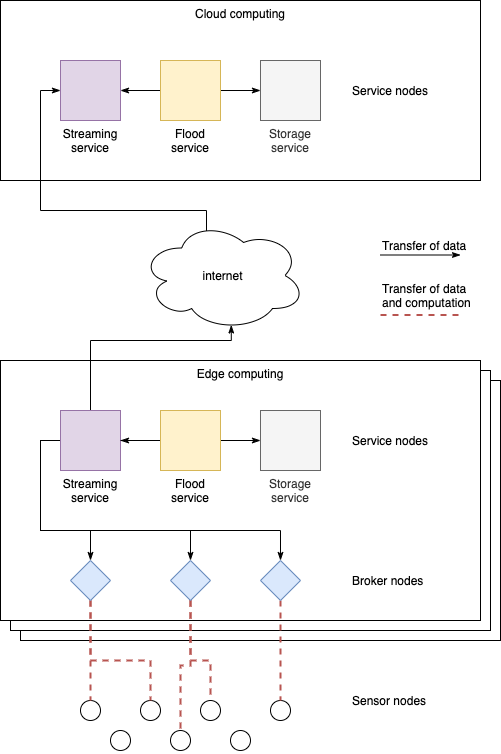
\includegraphics[width=\columnwidth]{figures/architecture-levee2}
\caption{Architecture for the flood warning system.}
\label{fig:architecture-levee}
\end{figure}

The application implements a system based on the architecture proposed in Figure~\ref{fig:architecture-levee}:

\begin{itemize}
    \item Sensor nodes: they are composed of sensor devices that collect data, preprocess it and transmit it to the edge cluster for further processing. One challenging task of this layer is implementing the dynamic configuration of the internal logic, as preprocessing can result in more accurate predictions, less bandwidth usage and more energy efficiency. The arbitrary code execution is safely enabled by running a WebAssembly interpreter on the Wasm binary file. The portable low-overhead Wasm format unlocks transfer of computation to dynamically instruct the sensor nodes about the preprocessing logic on a case-by-case basis;
    \item Broker nodes: they expose the sensor nodes behind a RESTful interface. \textcolor{red}{At this stage in Akri, each sensor node discovered by Kubernetes has an associated broker responsible for the communication with the rest of the services. However, a single broker should be able to aggregate the data from multiple sources.} The broker subscribes to the IoT REST resources via a CoAP message, and the device periodically sends CoAP updates, which are forwarded to the cluster as WebSocket packets. The broker ensures that both parts, IoT nodes and services nodes, are independent as far as they agree to communicate following the REST architecture. \textcolor{red}{Service nodes typically use REST over HTTP, while sensor nodes prefer CoAP};
    \item Service nodes: they implement the services needed by the flood warning system and allow them to be reused across different clusters. The use case needs a streaming service to aggregate the data from the device brokers, a local database to store the information for the analysis, and a flood prediction service to analyse the information and provide insight. 
\end{itemize}

The service nodes are deployed at multiple edge clusters, corresponding to different stations, and at a cloud cluster. The rationale for expanding the services to the cloud is two-fold.

First, the edge clusters are heterogeneous in computing capacity, and some zones may have not enough computing power to handle streams. Leveraging the cloud can help increase the workload at the cost of more bandwidth usage and latency. Such compromise might be acceptable, especially in the case of intensive data analysis on the sensor data.

Second, the prediction model could benefit from more knowledge derived from multiple streams geographically distributed. Likewise, a flood risk assessment model running in the cloud could achieve a globally optimal solution, whereas edge services can output only locally optimal results. On the other hand, during flood threat scenarios, the communication channels may become unavailable, so the system must perform a localised assessment. Unfortunately, the loss of communication is unpredictable, but the system must quickly adapt to the scenario. Such computing dynamism is a perfect scenario where the Continuum shines compared to relatively static cloud-only, edge-only, or pre-defined cloud+edge architectures.

\subsection{Evaluation of WebAssembly for microcontrollers}

\begin{figure}[ht]
\centering
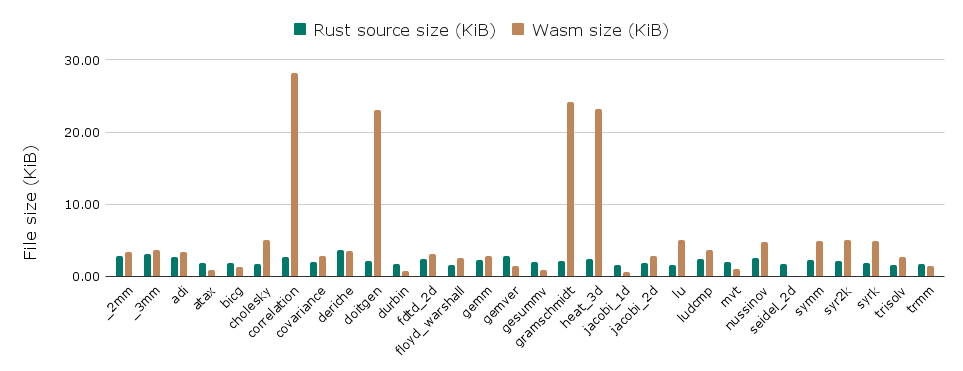
\includegraphics[width=\columnwidth]{figures/b-wasmi-2}
\caption{\textcolor{red}{Comparison of Wasm size (KiB) and Rust source size (KiB).}}
\label{fig:b-wasmi-2}
\end{figure}

\begin{figure}[ht]
\centering
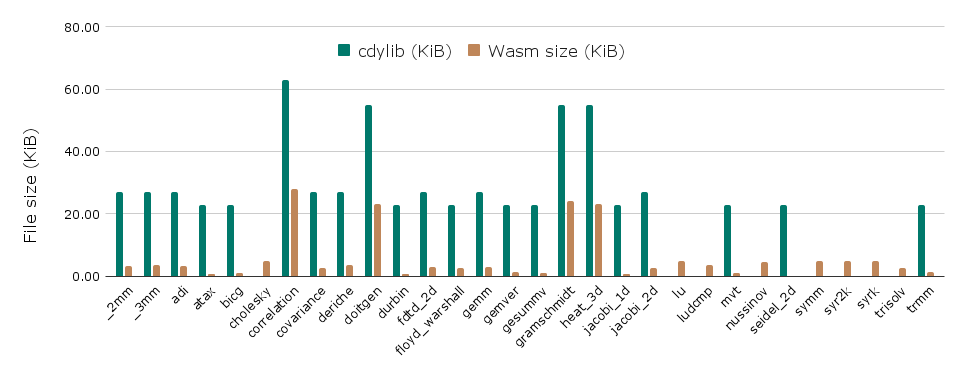
\includegraphics[width=\columnwidth]{figures/b-wasmi-3}
\caption{Comparison of Wasm size (KiB) and C dynamic library size (KiB).} \label{fig:b-wasmi-3}
\end{figure}

Figures~\ref{fig:b-wasmi-2} and~\ref{fig:b-wasmi-3} present a comparison of the sizes of different Wasm binaries compiled from the Polybench \cite{yuki2014understanding} modules. The Polybench benchmark suite offers relevant functions to embedded systems as it includes common matrix and statistical operations.

{\color{red}
Figure~\ref{fig:b-wasmi-2} offers a direct comparison of binary size and source size. However, comparing with source code is rarely meaningful due to factors including the widespread use of conditional compilation and unpredictable build behaviours. The purpose is to achieve an initial grasp of the Wasm binary size. The author has attempted to control for these effects by configuring the Rust toolchain to reasonable defaults. The compiler is configured to rely on LLVM to optimize the resulting code for code size. The toolchain also uses LLVM's link-time optimization (LTO) to ensure further size optimisation.

Once the compilation process is done, the result is a self-contained, sandboxed Wasm binary file ready for deployment onto the Continuum.

The results show how the final Wasm binary size has no predictable correlation to the source size, despite being usually about 2x larger, with some exceptions. Modules like "correlation" show a significant increase in the Wasm size relative to source code lines. Such a variety of differences depends on the source code's specific instructions and the toolchain configuration. Notably, loops, inlined functions and math functions can result in substantial differences in the output size because of the different optimisation techniques the compiler may take. Such unpredictability means that the Wasm toolchain is not immune to the compilers' famous idiosyncrasy, and developers must be careful always to check the final output.
}

This work has also chosen the C dynamic library size as a more meaningful comparison since it is a close alternative to Wasm binary files. Both outputs have been compiled using the same LLVM toolchain and optimisation flags. In such a case, the results undeniably favour the Wasm binary format as the C dynamic lib is often many times larger. The author has even removed some of the Polybench modules (namely \emph{cholesky, lu, ludcmp, nussinov, symm, syr2k, syrk, and trisolv}), which had a significantly larger C dynamic library size of 1.5MB (compared to about 5-10KiB in Wasm), which would make the other modules in the chart visually hard to evaluate. Comparing Wasm files to containers would greatly favour the former, as containers package a whole operative system filesystem. Even the smallest image base, "Alpine Linux Mini Root Filesystem", has an additional size of about 5.5MB uncompressed.

\begin{figure}[ht]
\centering
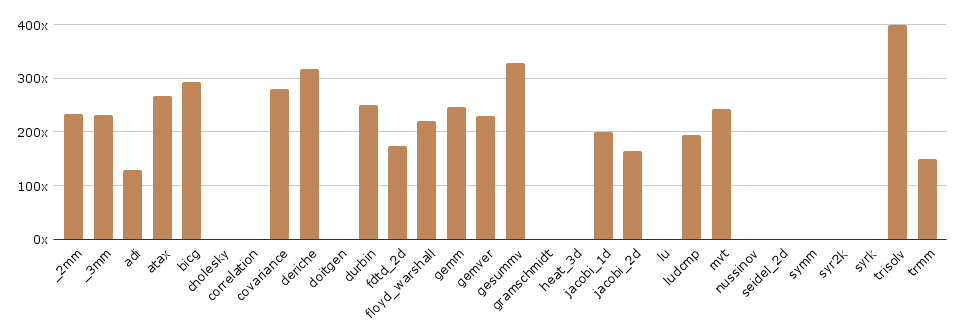
\includegraphics[width=\columnwidth]{figures/b-wasmi-4}
\caption{Comparison of Wasm interpreter performance and Rust native performance.} \label{fig:b-wasmi-4}
\end{figure}

Figure~\ref{fig:b-wasmi-4} offers an overview of the Wasm interpreter's execution performance on the STM32F407 microcontroller. Each Polybench benchmark has been run 15 times, following the same methodology described in \cite{wasm3-performance}. The results show a dramatic slowdown compared to the Rust native alternative, with a factor of 100-400 times. Such results are discouraging for the idea of using Wasm interpreters on microcontrollers to support dynamic reconfiguration.

However, it is fair to note that the Wasm interpreter wasmi \cite{wasmi} was adapted to work on embedded devices and was not designed for highly constrained devices. wasmi is developed by Parity, a blockchain company, and is thus used to offer a deterministic sandboxed execution context running on cloud servers. As a result, execution performance is not paramount, unfortunately. The alternative interpreter wasm3, implemented in the C language, shows a much minor execution penalty, in the order of 30-60x slower than native \cite{peach2020ewasm}. Thus, it is reasonable to believe that future efforts may allow a comparable result for the Rust-built wasmi interpreter. Nevertheless, 30x times execution over time can still arguably deter the usage of interpreters in microcontrollers. Future work should also provide a benchmark with respect to other popular interpreted languages like Lua, Python, and JavaScript.

\begin{figure}[ht]
\centering
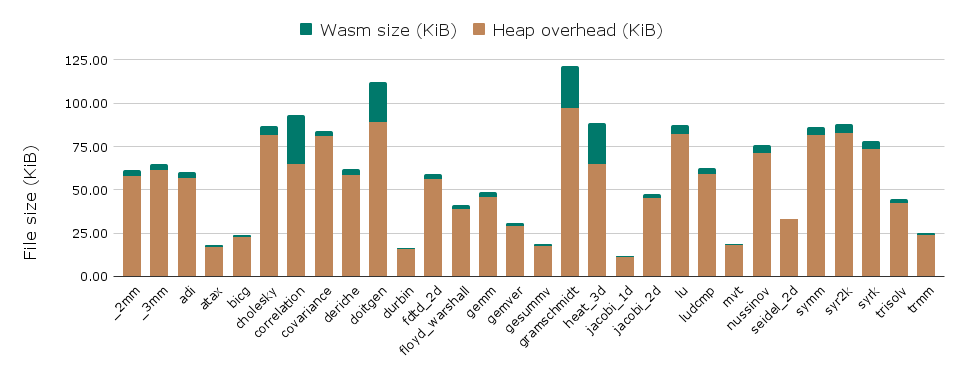
\includegraphics[width=\columnwidth]{figures/b-wasmi-1}
\caption{Comparison of Wasm size (KiB) and heap overhead (KiB).}
\label{fig:b-wasmi-1}
\end{figure}

As an additional benchmark, the author has evaluated the heap overhead of interpreting Wasm on microcontrollers. 
Figure~\ref{fig:b-wasmi-1} presents a significant increase in the heap usage with respect to the Wasm size. However, the most crucial concern is that such a heap increase is not predictable. Such unpredictability does not come in favour of the usage of WebAssembly on microcontrollers, as embedded devices have extremely limited resources and must have predictable behaviours to ensure proper real-time execution. Such deficiency is an intrinsic issue with interpreters, as the code instructions and execution data structures must be stored in heap memory. This behaviour contrasts with the binary executables that can save and access instructions or read-only data on the more capable flash storage. Writable data is saved in the stack instead, and it can be calculated with accuracy in many production-grade toolchains like C and Ada.

Generally speaking, running Wasm on resource-constrained microcontrollers has also presented other challenges.

\begin{itemize}
    \item Memory architecture: Wasm's 64 KiB pages are too large for microcontrollers that often have between 16-256 KiB SRAM. Dynamic allocation is a common requirement even for embedded systems. However, Wasm specifies that the sandbox should expand the memory by 64KiB chunks, which is not granular enough for constrained embedded systems. As a consequence, the wasmi interpreter has been modified to allocate non-standard pages of 16KiB. Otherwise, it would have been impossible to execute any benchmark on the STM32F407 microcontroller, as additional heap space is required for the interpreter's internal structures and the Wasm instructions themselves. There is a need for a Wasm embedded standard that supports smaller granularity of memory pages;
    \item \textcolor{red}{Assumed floating-point operations: Wasm specifically is a 32-bit virtual architecture and supports floating-point, but not all Cortex-Ms do. In such cases, floating-point emulation must be provided by the programmer. In Rust, this solution is typically accomplished utilising the \emph{libm} library, a port of MUSL's libm containing the most popular math operations. MUSL is a lightweight alternative to the conventional libc and employed as an alternative in Alpine Linux. However, the Rust ecosystem is less mature and complete on this matter than the C version, and the many floating-point functions are still missing in libm.} 
\end{itemize}

% \subsection{Evaluation of CoAP for microcontrollers}

% \begin{figure}[ht]
% \centering
% 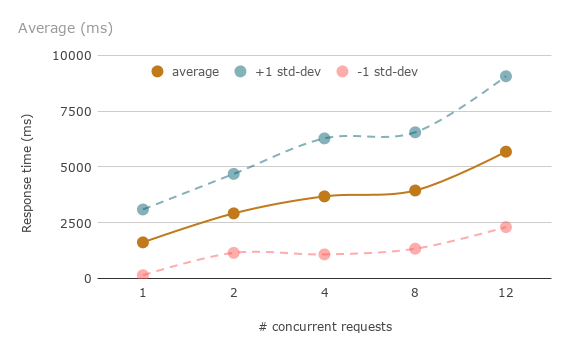
\includegraphics[width=\columnwidth]{figures/b-coap-1}
% \caption{Average response time for concurrent CoAP requests \label{fig:b-coap-1}}
% \end{figure}

% \begin{figure}[ht]
% \centering
% 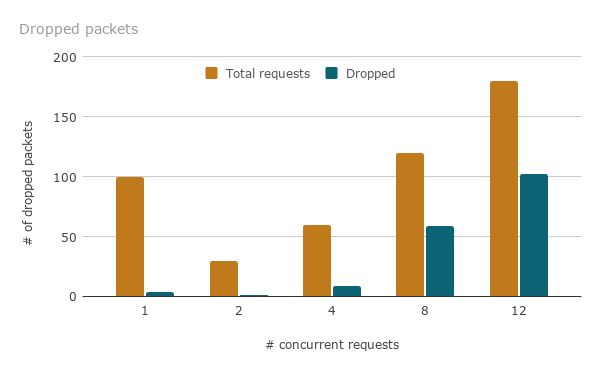
\includegraphics[width=\columnwidth]{figures/b-coap-2}
% \caption{Number of dropped packets as concurrency increases \label{fig:b-coap-2}}
% \end{figure}

% Fig. \ref{fig:b-coap-1} and Fig. \ref{fig:b-coap-2} present the experimental evaluation of the CoAP implementation in Rust. The STM32F407 is equipped with a LAN8720 ETH 10/100Mbs module connected to the microcontroller via cheap jumper wires. On the software stack, the device offers a CoAP server running on the RTIC runtime. Such a server is put under stress by firing concurrent requests from a machine connected to the same network, and the test is repeated 15 times. As expected, the response times increase as the number of concurrent requests rises. However, such escalation of response time is not exponential and presents a good smoother curve. The standard deviation range is also significantly large, as the embedded device cannot provide timely responses. Further experiments should compare the CoAP server with an equivalent HTTP or MQTT server running on the same RTIC runtime.

% On a different note, the number of dropped packets dramatically increases as the concurrency grows. Such behaviour is expected, and the experimental logs provide a plausible rationale. As the number of concurrent requests increases, the microcontroller network buffers cannot cope with the volume, and the packets are even truncated before being parsed. A deeper analysis should check whether the issue can be solved by allocating more buffer space or, on the contrary, is a hardware-related limit. Admittedly, the hardware network connection via jumper wires is not the most robust solution.

\subsection{Evaluation of Wasm as virtualisation technology}

The following benchmarks measure how long it takes to create and boot a Wasm-based Kubernetes Pod, how the memory scales as the number of running Pods increases, and how both metrics compare to containers. The benchmark is a simple DateTime application that logs the current system time upon creation and goes into sleep. By going to sleep, the Pod does not complete, and the resources remain allocated. The log is later retrieved using the Kubernetes API to calculate the boot time. 

Wasm Pods run on Krustlet \cite{krustlet}, whereas container Pods are scheduled on the K3s \cite{k3s} Kubelet. Krustlet (a Kubernetes-Rust-Kubelet) is an experimental implementation of the Kubelet APIs that supports Wasm as virtualisation technology. It is designed to run as a Kubernetes Kubelet. Therefore, it listens to the Kubernetes API event stream for new Pods and runs them under a WebAssembly System Interface (WASI) runtime (notably, Wasmtime by Mozilla \cite{wasmtime}).

On the other hand, K3s is a fully certified Kubernetes distribution geared towards resource-constrained environments backed by a commercial company. K3s is implemented in Go and packaged as a single binary of about 50MB in binary size. It bundles everything needed to run Kubernetes, \textcolor{orange}{notably the container runtime.} \textcolor{red}{, including the container runtime (namely containerd \cite{containerd}), a Container Network Interface implementation (Flannel \cite{flannel}), a DNS server (CoreDNS \cite{coredns}), and a simple ingress load balancer (Traefik \cite{traefik}). The OS dependencies are also minimal and well supported by all the modern Linux distributions.}

\textcolor{red}{Krustlet has been customised to measure the time it starts to instantiate the Pod's necessary Wasm runtime. On the other hand, K3s and Kubernetes do not provide tools explicitly meant to obtain such value, and the author does not have the Go knowledge to modify and re-compile K3s. As a result, the start time is collected from the Kubernetes Pod metrics, which provides the time at which the Kubelet receives the request to provision the container. The provision request is followed by the container image's pull and then instantiation of the container itself. To avoid counting the additional image pull time, the author has explicitly configured the Pod to use the cached image and ensured that the Kubelet always has such cache. Lastly, the granularity of the Kubernetes start time metric is only up to seconds.}

\begin{figure}[ht]
\centering
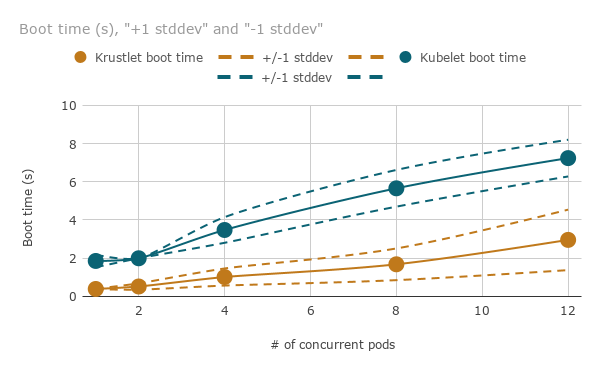
\includegraphics[width=\columnwidth]{figures/b-krustlet-1}
\caption{Average boot time for concurrent Wasm Pods.}
\label{fig:b-krustlet-1}
\end{figure}

Figure~\ref{fig:b-krustlet-1} shows the average boot time, along with the standard deviation, of both the Kubernetes Pods containing Wasm binaries and the conventional Pods containing containers. The benchmark concurrently deploys the Pods and repeats the process 15 times. Pods are not deleted between iterations, so that increasing memory utilisation is also collected.

The experimental results show that a Wasm-based virtualisation strategy incurs less boot time. However, the more mature container Kubelet presents a more linear curve and minor standard deviation as the number of concurrent deployments increases. Because efficient concurrency is essential as much as a fast boot time, there is no clear winner. Nevertheless, such preliminary results encourage the idea of adopting Wasm as an alternative to container technology since efficiency was not a primary design goal in the early implementations of Krustlet and Wasmtime. Future versions will probably provide even more competitive results.

\begin{figure}[ht]
\centering
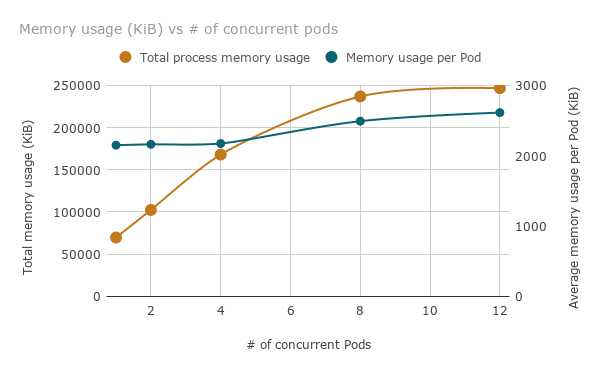
\includegraphics[width=\columnwidth]{figures/b-krustlet-2}
\caption{Average memory usage of concurrent Wasm.}
Pods \label{fig:b-krustlet-2}
\end{figure}

\begin{figure}[ht]
\centering
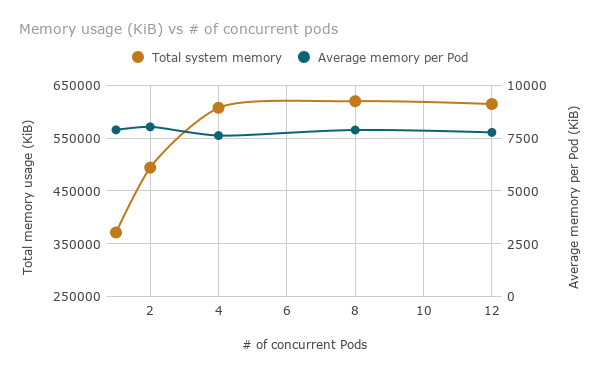
\includegraphics[width=\columnwidth]{figures/b-krustlet-3}
\caption{Average memory usage of concurrent K3s Kubelet Pods.}
\label{fig:b-krustlet-3}
\end{figure}

Figures~\ref{fig:b-krustlet-2} and~\ref{fig:b-krustlet-3} offer an overview of the memory overhead of the two different virtualisation solutions. \textcolor{red}{The memory utilisation has been tracked using the Linux \emph{pmap} utility, which allows the granular analysis of the system memory allocated by a process. In Krustlet's case, the task is trivial as Wasm modules run in the same process as the host, and only additional Pods can significantly increase the heap memory, as Rust is not garbage collected. On the contrary, K3s instantiates a process for each new container. It is much more difficult to evaluate each Pod's memory cost, as the Go language uses the heap for every aspect. Therefore, in the latter case, we resort to measuring the system memory using the Linux \emph{free} program. Fortunately, since the author uses Alpine Linux with a minimal configuration to support just enough to run Kubernetes, the system measurements are relatively free from other processes' contamination.}

In such a comparison, Wasm Pods are the winners in memory usage per Pod unit, but the K3s Kubelet can achieve higher total memory utilisation. Notably, the K3s Kubelet can completely use the available memory until the machine cannot even function properly. On the other hand, the Krustlet node fails to allocate new Pods even when there is sufficient memory space. The allocation results in an Out Of Memory error, and the node is still completely functional. To the best of the authors' knowledge, the potential cause is the Rust vector allocation strategy, which doubles the capacity when its current limit is reached. \textcolor{red}{As a result, when Krustlet's heap reaches about 256MB, the process demands the kernel an additional 512MB of space. Such demand cannot be met, and the Rust runtime returns an Out Of Memory error. Further analysis of the Wasmtime implementation is needed to validate this hypothesis.}

On a different note, as Go is a garbage-collected language, the heap utilisation is highly unpredictable. \textcolor{red}{The Go Garbage Collector (GC) uses a pacer to determine when to trigger the next GC cycle \cite{go-gc}. Pacing is modelled like a control problem where it is trying to find the right time to trigger a GC cycle to hit the target heap size goal. Go’s default pacer will try to trigger a GC cycle every time the heap size doubles. The net result is that the K3s increase memory usage even during idle periods, as it processes the ordinary Kubernetes operations to maintain functionality.} Besides, as the GC kicks in only when the heap size doubles, the hardware memory is underutilised. The freeable memory should be used for running additional pods, achieving better Pod packing. Such efficiency is crucial for edge nodes that have already limited hardware capabilities but must support multiple workloads. This consideration is another point favouring the adoption of the Rust language to develop the Continuum infrastructure. \textcolor{red}{Table \ref{tab1} presents the system memory utilisation during an idle state.}

\textcolor{red}{Finally, in both technologies, the memory overhead per Pod is relatively constant. However, the Wasm Pod incurs approximately 2x-3x less overhead, allowing more efficient packing of applications on the same machine. For example, the Raspberry Pi 3B+ can support up to 80 Wasm Pods and still have 500MB of free memory (although no more Pods can be allocated). In contrast, the K3s Kubelet achieves maximum memory utilisation of about 55 container Pods, and the entire node becomes completely unresponsive. The author believes that such results pledge to favour Krustlet, as the premature Out Of Memory error can be fixed on later Wasmtime versions. In contrast, the container overhead is already the state of the art of a decade of research in container technologies.}

\begin{table}
\caption{\textcolor{red}{Memory usage of Kubernetes on edge Raspberry Pi.}}
\begin{tabular}{|l|l|}
\hline
Software stack & Idle memory usage \\
\hline
Alpine Linux 3.12.1 & ~50MB \\
Alpine Linux + K3s master & ~304MB \\
Alpine Linux + K3s agent & ~110MB \\
Alpine Linux + Krustlet & ~120MB \\
\hline
\end{tabular}
\label{tab1}
\end{table}

\subsection{Evaluation of Wasm for Machine Learning}

In the field of machine learning, numerical precision matters. WASM natively supports floating-point arithmetic, whereas other popular machine learning backends like WebGL requires hardware extensions. Not all devices support this extension, which means a GPU-accelerated machine learning is not supported on some devices (e.g. older mobile devices which can run Wasm instead).

Moreover, GPU drivers can be hardware-specific and different devices can have precision problems. \textcolor{red}{On iOS, 32-bit floats are not supported on the GPU. Consequently, TensorFlow \cite{tensorflow}, the popular machine learning library developed by Google, falls back to 16-bit floats, causing precision problems.} In WASM, computation always happens in 32-bit floats and thus have precision parity across all devices. Such numerical predictability is also paramount in blockchain applications \textcolor{red}{, as proved by Parity's interest in WebAssembly} \cite{parity-wasm}.

The author has compiled the flood prediction model to Wasm: Figure~\ref{fig:b-krustlet-4} evaluates the model's response time with increasing concurrency. The flood prediction model is a conventional Deep Neural Network constituted by three dense layers of 32, 16 and 1 units. The model has been trained on the cloud using the traditional machine learning framework Keras \cite{keras}. Keras provides a Python interface for artificial neural networks on top of the TensorFlow library.

As of the time of writing, TensorFlow provides a WebAssembly (WASM) backend for both the browser and Node.js \cite{tf-wasm}. However, the library itself cannot be easily compiled to WebAssembly yet, to the best of the authors' knowledge. As a result, the trained Keras model is saved to the ONNX \cite{onnx} standard format and executed by the \emph{tract} library \cite{tract}. tract is a Rust neural network inference library that can read Tensorflow or ONNX models and run data through them. It also supports compilation to Wasm as a target. The resulting Wasm module exports a public function through which Krustlet can pass the model inputs. 

At the time of writing, it has not been possible to implement a web server directly on top of the inference model and compile the application to Wasm. There is an underlying issue with implementing network servers with Wasm as there is neither complete network nor multi-threading support yet.

First, the current WebAssembly System Interface (WASI) standard only contains a few methods for working with sockets that are not enough for complete networking support. Adding support for connecting to sockets is fundamental to allow Wasm modules to connect to web servers, databases, or any service. As a workaround, this paper has implemented the capability to invoke functions in Wasm Pods on top of the Kubernetes \emph{exec} API \cite{k8s-exec}, which is however designed to execute commands in a container from the Kubernetes command line, and it is an undocumented interface. \textcolor{red}{Besides, as WASI lacks network APIs and Krustlet does not support the Kubernetes networking configuration yet, the POC uses a hybrid approach where conventional Kubelets with container runtimes are used as a fallback.}

Second, the lack of concurrency primitives means that a server running in WebAssembly is single-threaded, or its implementation has to be significantly more complex (e.g. Node.js's event loop). This limitation severely narrows the workload capabilities of the server. At the time of writing, the WASM spec has outlined a thread and atomics proposal intending to speed up multi-threaded applications. The proposal is still in the early stage, and it is implemented only in web browsers, behind an experimental flag.

\begin{figure}[ht]
\centering
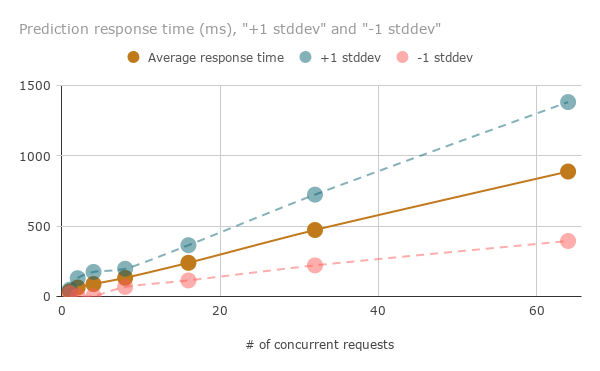
\includegraphics[width=\columnwidth]{figures/b-krustlet-4}
\caption{\textcolor{red}{Latency of the Wasm flood prediction model with varying concurrency.}} \label{fig:b-krustlet-4}
\end{figure}

\textcolor{red}{Figure~\ref{fig:b-krustlet-4} illustrates the flood prediction response times within a Wasm Pod in the same fashion of serverless functions. As expected, the response times increase linearly with varying concurrency. Because the WASI standard does not support multi-threading, the requests are completed sequentially.}

\section{Conclusion}
\label{sec:conclusion}

This paper has presented a computing continuum vision and the challenges that the industrial and academic community will face implementing such a paradigm. The author has also presented a candidate architecture for the infrastructure and implemented a Proof of Concept based on the technologies available at the time of writing. Such POC has been applied to a real-world use case of flood prediction as well. The net result is a working prototype based on the presented architectural and software concepts. The implementation is publicly available on GitHub \cite{fedra-thesis}. 

In the authors' view, we are clearly at a convergence point after the last decades of technological advances. However, a significant number of challenges (§\ref{sec:challenges}) lie ahead the path to the realisation of the Continuum.

The WebAssembly standard is a potential enabling technology, but it is still in its infancy. As shown by the experimental results, WebAssembly is mainly suited for pure computational functions. The lack of multi-threading and a mature network interface severely limit the space of real-world applications. Most of the production use cases of WebAssembly involve pure computation scenarios, typically machine learning and relatively simple serverless functions. Some projects try to overcome the API limitations by providing custom system capabilities, to the detriment of the platform-independency feature of WebAssembly, unfortunately.

{\color{red}
Results show that Wasm-based Pods in Krustlet incur fixed low overhead in memory usage and competitive boot times compared to more mature container solutions. The outcome is intriguing as these technologies (Krustlet and Wasmtime) are still in their infancy.

As a concluding note, although the proposed architecture and the related technologies are still very immature, they open up a set of exciting opportunities for the Continuum's realisation.
}
